\chapter{Background Estimation}
\label{background}
\label{backgrounds}

Perhaps the most critical aspect of a physics analysis is estimating the background contribution in the data sample. Most physics backgrounds can be modeled using simulated Monte Carlo events and the rest are modeled using reconstructed data events. This chapter describes how all backgrounds are modeled and normalized to their expected contribution in the dataset. Section~\ref{backgroundmodel} describes the expected backgrounds in the single top quark dataset and how the background event kinematics are modeled. Section~\ref{backgroundnorm} describes how these backgrounds are normalized to their expected yields in the dataset. Finally, Section~\ref{backgroundyields} summarizes all background yields and Section~\ref{databackcompare}~compares data with the expected background estimation.

\section{Background Modeling}
\label{backgroundmodel}

As described in Chapter~\ref{theory} the top quark in single top quark events will decay to a $W$ boson and $b$ quark, where the $W$ boson is only considered to decay to a lepton and neutrino in this analysis\footnote{$t\rightarrow bW \rightarrow bqq^{'}$ decays are removed from the dataset since there is no lepton nor large missing $E_{T}$.}. With an additional $b$ quark or light quark this makes the signature of single top quark events one high $p_{T}$ lepton, large missing $E_{T}$, and two or more jets. This event signature can be produced by three general types of backgrounds. The largest background which produces this event signature is $W$ or $Z$ boson production in association with two or more jets. Because the kinematics of $Z$ boson production are similar to $W$ boson production, both backgrounds are typically considered as one background called ``$W$+jets". An example Feynman diagram for such a process is shown in Fig.~\ref{wjetsexample}.

\begin{figure}[!h!tbp]
\begin{center}
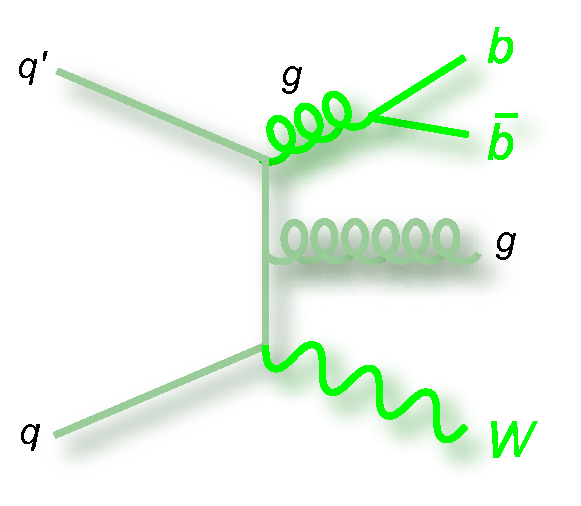
\includegraphics[width=0.5\textwidth]{eps/Feynman/feynman_Wbbg.eps}
\end{center}
\vspace{-0.1in}
\caption{Example leading order Feynman diagram for a ``$W$+jets" event. This particular diagram represents the production of a $W$ boson, and two $b$~quarks and an associated gluon~\cite{feynmandiagrams}.}
\label{wjetsexample}
\end{figure}

Another large background present in the dataset are events origination from top pair production. The top pair production background, referred to as $\ttbar$, is defined by the decay of the two $W$ bosons, from the decay of the two top quarks. The first case when one of the $W$ bosons decays to two quarks and other decays to a lepton and neutrino is referred to as ``lepton+jets" ($\lepjets$) because the final state in the event is one lepton, one neutrino, and four quarks. The other way in which a $\ttbar$~event can enter the data sample is when both $W$ bosons decay to leptons and neutrinos. In this case, there are two quarks, two leptons, and two neutrinos. These events are referred to as ``dilepton'' ($\dilepton$) events. An example Feynman diagram for the $\lepjets$~process is shown in Fig.~\ref{ttbarexample}.

\begin{figure}[!h!tbp]
\begin{center}
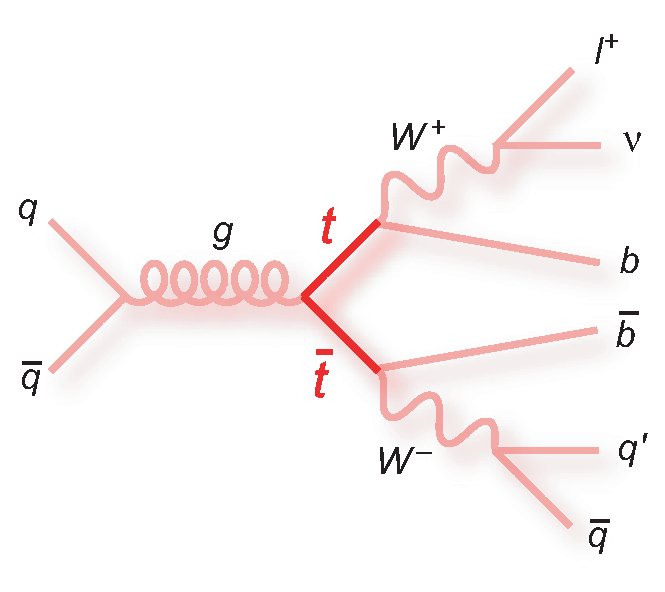
\includegraphics[width=0.5\textwidth]{eps/Feynman/feynman_ttbar_ljets.eps}
\end{center}
\vspace{-0.1in}
\caption{Example Feynman diagram for a $\lepjets$ event~\cite{feynmandiagrams}.}
\label{ttbarexample}
\end{figure}

The third largest background present in the dataset is multijet events produced by the strong interaction. The background processes responsible for these events in the dataset are quite different for electron events and muon events. In electron events one of the reconstructed jets will have a large electromagnetic fraction causing it to be mis-identified as an electron. In muon events a gluon will decay to a $b\bar{b}$ pair and one of the $B$ mesons will undergo a semi-leptonic decay and produce a muon. In both cases, another jet may not be properly reconstructed leading to a large amount of missing E$_{T}$ in the event, thus mimicking the single top quark event signature. An example Feynman diagram for a multijet process producing a lepton, missing E$_{T}$, and jets is shown in Fig.~\ref{qcdexample}.

\begin{figure}[!h!tbp]
\begin{center}
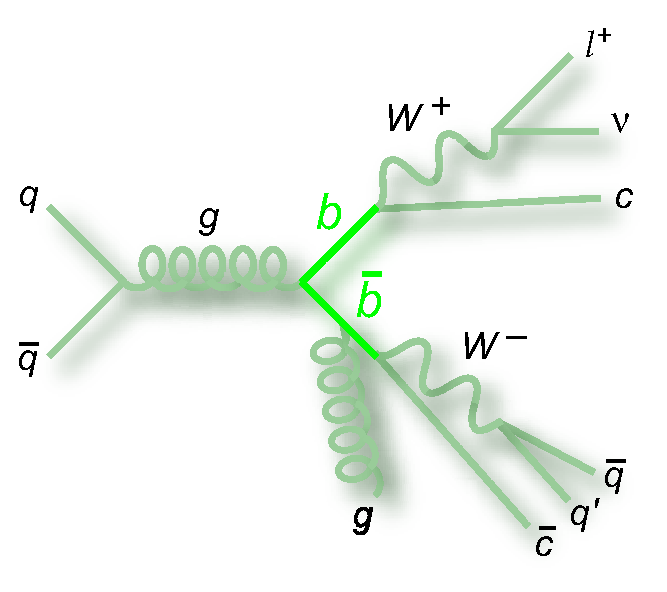
\includegraphics[width=0.5\textwidth]{eps/Feynman/feynman_bbbar_ljets.eps}
\end{center}
\vspace{-0.1in}
\caption{Example Feynman diagram for a multijet event~\cite{feynmandiagrams}.}
\label{qcdexample}
\end{figure}


\subsection{Monte Carlo Modeling of W + Jets and $\ttbar$ Backgrounds}
\label{wjetsmodel}
$W$+jets and $\ttbar$ backgrounds are modeled using the ALPGEN Monte Carlo generator interfaced with Pythia for parton showering~\cite{Mangano:2002ea}. ALPGEN is a leading order matrix element Monte Carlo generator similar to the CompHEP generator used to model single top quark events. All generated events are reconstructed using the simulated $\dzero$~detector as described in Chapter~\ref{EventSelection} and selection cuts are applied as described in Chapter~\ref{analysis}. Within ALPGEN, the MLM jet-parton matching scheme~\cite{Hoche:2006ph} is also employed to remove double counted events in a similar manner to the double counting that is encountered when generating single top events. An example of double counting in $W$+jets events is given here: $W$+light flavor events (e.g $Wgg$) are generated separately from $W$+heavy flavor events (e.g $Wbb$). When these events are sent through Pythia it is possible that addition gluons will split to heavy flavor quarks (e.g $g\rightarrow b\bar{b}$) leading to double counting of $W$+heavy flavor events. The MLM matching scheme is described in more detail below.

\subsubsection{MLM Matching Scheme}

As stated earlier, the MLM jet-parton matching scheme is designed to remove double counted events. The MLM matching scheme works in the following way:

\begin{enumerate}
\item Events are generated with a distinct parton multiplicity. For instance, $W$+2 light partons (e.g. $Wgg$) are generated separately from $W$+3 light partons (e.g. $Wggg$). The same applies to $W$+heavy flavor and $\ttbar$~events.
\item All generated events are sent to Pythia for parton showering. This procedure will introduce additional quarks and gluons as a product of the shower.
\item Before the final state partons are hadronized, all quarks and gluons are clustered together with a jet algorithm. The algorithm used for this analysis is the UA1 jet cone algorithm~\cite{PhysRevLett.54.1983}.
\item Match the generated partons from (1) with the cone jets from (3). Each parton must correspond to one jet and visa versa. A jet is matched if it has p$_{T}>15$~GeV and there is a parton with $\Delta R<0.7$ from the jet. If a match is found the event is kept, otherwise the process is repeated.
\item Combine all samples together with weights based on the relative cross sections and the relative number of generated events for each process. 
\end{enumerate}

The formulas used to combined $W$+light parton, $W$+$c\bar{c}$+light parton, $W$+$b\bar{b}$+light parton, $\dilepton$+light parton, and $\lepjets$+light parton events are shown below.

\subsubsection{$W$+Light Parton Sample}

The $W$+light parton sample contains $W$+light flavor ($udsg$) events as well as $W$+$c$+light flavor events. In $W$+$c$+light flavor events the $c$-quark is considered massless. Eq.~\ref{wlp} shows the formula used to combine the $W$+light parton sample and Table~\ref{wjjcross} shows the relative cross sections and weights (k) for each sample. All $W$+light parton events are generated using CTEQ6L1 PDFs with $Q^{2}=m_{W}^{2} + P^{2}_{T}(W)$.

\begin{eqnarray}
\label{wlp}
\nonumber
W+\rm{Nlp} &=& k_{W+0\rm{lp}} \left[W+0\rm{lp}\right]_{\rm{excl}} + k_{W+1\rm{lp}} \left[W+1\rm{lp}\right]_{\rm{excl}} + \\
\nonumber
& & k_{W+2\rm{lp}} \left[W+2\rm{lp}\right]_{\rm{excl}} + k_{W+3\rm{lp}} \left[W+3\rm{lp}\right]_{\rm{excl}} + \\
& & k_{W+4\rm{lp}} \left[W+4\rm{lp}\right]_{\rm{excl}} + k_{W+5\rm{lp}} \left[W+5\rm{lp}\right]_{\rm{incl}}	\\
\nonumber
\end{eqnarray}



\begin{table}[!h!tbp]
\begin{center}
\caption{Absolute weights for $W$+light parton ALPGEN Monte Carlo events.}
\label{wjjcross}
\begin{tabular}{c|cccc}
%\multicolumn{5}{c}
%{\underline{Absolute Weights For $W$+Light Parton ALPGEN Monte Carlo Events}} \\
Sample			&	Type		&	Cross Section [pb]	&	Events	&	Weight (k) \\
\hline
$k_{W+0\rm{lp}}$	&	Exclusive	&	$4574$			&	7844750	&	$2.15$			\\
$k_{W+1\rm{lp}}$	&	Exclusive	&	$1273$			&	1053000	&	$0.68$			\\
$k_{W+2\rm{lp}}$	&	Exclusive	&	$298.5$			&	1250500	&	$0.34$	\\
$k_{W+3\rm{lp}}$	&	Exclusive	&	$70.56$			&	621000	&	$16.4$	\\
$k_{W+4\rm{lp}}$	&	Exclusive	&	$15.83$			&	582250	&	$0.07$	\\
$k_{W+5\rm{lp}}$	&	Inclusive	&	$11.29$			&	41750	&	$0.13$
\end{tabular}
\vspace{-0.1 in}
\end{center}
\end{table}

\subsubsection{$W$+$c\bar{c}$+Light Parton Sample}

The $W$+$c\bar{c}$+light parton sample contains $W$+$c\bar{c}$ (from gluon splitting) + light flavor partons. In contrast to the $W$+light parton samples the $c$-quark in these events are massive. Eq.~\ref{wcc} shows the formula used to combine the $W$+$c\bar{c}$+light parton sample and Table~\ref{wcccross} shows the relative cross sections and weights (k) for each sample. All $W$+$c\bar{c}$+light parton events are generated using CTEQ6L1 PDFs with $Q^{2}=m_{W}^{2} + P^{2}_{T}(W)$.

\begin{eqnarray}
\label{wcc}
\nonumber
W+c\bar{c}+\rm{Nlp} &=& k_{W+c\bar{c}+0\rm{lp}} \left[W+c\bar{c}+0\rm{lp}\right]_{\rm{excl}} + k_{W+c\bar{c}+1\rm{lp}} \left[W+c\bar{c}+1\rm{lp}\right]_{\rm{excl}} + \\
& & k_{W+c\bar{c}+2\rm{lp}} \left[W+c\bar{c}+2\rm{lp}\right]_{\rm{excl}} + k_{W+c\bar{c}+3\rm{lp}} \left[W+c\bar{c}+3\rm{lp}\right]_{\rm{incl}}
\end{eqnarray}


\begin{table}[!h!tbp]
\begin{center}
\caption{Absolute weights for $W$+$c\bar{c}$+light parton ALPGEN Monte Carlo events.}
\label{wcccross}
\begin{tabular}{c|cccc}
%\multicolumn{5}{c}
%{\underline{Absolute Weights For $W$+$c\bar{c}$+Light Parton ALPGEN Monte Carlo Events}} \\
Sample					&	Type		&	Cross Section [pb]	&	Events	&	Weight (k) \\
\hline
$k_{W+c\bar{c}+0\rm{lp}}$	&	Exclusive	&	$71.15$			&	481572	&	$0.039$			\\
$k_{W+c\bar{c}+1\rm{lp}}$	&	Exclusive	&	$29.85$			&	336400	&	$0.036$			\\
$k_{W+c\bar{c}+2\rm{lp}}$	&	Exclusive	&	$10.25$			&	332347	&	$0.016$	\\
$k_{W+c\bar{c}+3\rm{lp}}$	&	Inclusive	&	$18.39$			&	372248	&	$0.020$	\\
\end{tabular}
\vspace{-0.1 in}
\end{center}
\end{table}

\subsubsection{$W$+$b\bar{b}$+Light Parton Sample}

The $W$+$b\bar{b}$+light parton sample contains $W$+$b\bar{b}$ (from gluon splitting) + light flavor partons. Eq.~\ref{wjetsbbsample} shows the formula used to combine the $W$+$b\bar{b}$+light parton sample and Table~\ref{wbbcross} shows the relative cross sections and weights (k) for each sample. All $W$+$b\bar{b}$+light parton events are generated using CTEQ6L1 PDFs with $Q^{2}=m_{W}^{2} + P^{2}_{T}(W)$.


\begin{eqnarray}
\label{wjetsbbsample}
\nonumber
W+b\bar{b}+\rm{Nlp} &=& k_{W+b\bar{b}+0\rm{lp}} \left[W+b\bar{b}+0\rm{lp}\right]_{\rm{exbl}} + k_{W+b\bar{b}+1\rm{lp}} \left[W+b\bar{b}+1\rm{lp}\right]_{\rm{exbl}} + \\
& & k_{W+b\bar{b}+2\rm{lp}} \left[W+b\bar{b}+2\rm{lp}\right]_{\rm{exbl}} + k_{W+b\bar{b}+3\rm{lp}} \left[W+b\bar{b}+3\rm{lp}\right]_{\rm{incl}}
\end{eqnarray}

\begin{table}[!h!tbp]
\begin{center}
\caption{Absolute weights for $W$+$b\bar{b}$+light parton ALPGEN Monte Carlo events.}
\label{wbbcross}
\begin{tabular}{c|cccc}
%\multicolumn{5}{c}
%{\underline{Absolute Weights For $W$+$b\bar{b}$+Light Parton ALPGEN Monte Carlo Events}} \\
Sample					&	Type		&	Cross Section [pb]	&	Events	&	Weight (k) \\
\hline
$k_{W+b\bar{b}+0\rm{lp}}$	&	Exclusive	&	$19.18$			&	738761	&	$0.014$			\\
$k_{W+b\bar{b}+1\rm{lp}}$	&	Exclusive	&	$7.939$			&	261300	&	$0.011$			\\
$k_{W+b\bar{b}+2\rm{lp}}$	&	Exclusive	&	$2.636$			&	171411	&	$0.005$	\\
$k_{W+b\bar{b}+3\rm{lp}}$	&	Inclusive	&	$1.742$			&	163674	&	$0.003$	\\
\end{tabular}
\vspace{-0.1 in}
\end{center}
\end{table}



\subsubsection{$\lepjets$+Light Parton Sample}

The $\lepjets$+light parton sample contains $\lepjets$ + light flavor partons. Eq.~\ref{ttbarsample} shows the formula used to combine the $\lepjets$+light parton sample and Table~\ref{lepjetscross} shows the relative cross sections and weights (k) for each sample. All $\lepjets$ events are generated using CTEQ6L1 PDFs with scale $Q^{2}=m_{t}^{2} + \sum_{\rm{jets}}P^{2}_{T}$.

\begin{eqnarray}
\label{ttbarsample}
\nonumber
\lepjets+Nlp&=& k_{\lepjets+0\rm{lp}} \left[\lepjets+0\rm{lp}\right]_{\rm{excl}} +\\
\nonumber
& & k_{\lepjets+1\rm{lp}} \left[\lepjets+1\rm{lp}\right]_{\rm{excl}} + \\
& & k_{\lepjets+2\rm{lp}} \left[\lepjets+2\rm{lp}\right]_{\rm{incl}} 
\end{eqnarray}


\begin{table}[!h!tbp]
\begin{center}
\caption{Absolute weights for $\lepjets$+light parton ALPGEN Monte Carlo events.}
\label{lepjetscross}
\begin{tabular}{c|cccc}
%\multicolumn{5}{c}
%{\underline{Absolute Weights For $\lepjets$+Light Parton ALPGEN Monte Carlo Events}} \\
Sample				&	Type		&	Cross Section [pb]	&	Events	&	Weight (k) \\
\hline
$k_{\lepjets+0\rm{lp}}$	&	Exclusive	&	$1.284$			&	283463	&	$0.048$			\\
$k_{\lepjets+1\rm{lp}}$	&	Exclusive	&	$0.625$			&	98425	&	$0.032$			\\
$k_{\lepjets+2\rm{lp}}$	&	Inclusive	&	$0.398$			&	92517	&	$0.020$			\\
\end{tabular}
\vspace{-0.1 in}
\end{center}
\end{table}



\subsubsection{$\dilepton$+Light Parton Sample}

The $\dilepton$+light parton sample contains $\dilepton$ + light flavor partons. Eq.~\ref{ttbardilepsample} shows the formula used to combine the $\dilepton$+light parton sample and Table~\ref{dileptoncross} shows the relative cross sections and weights (k) for each sample. All $\dilepton$ events are generated using CTEQ6L1 PDFs with scale $Q^{2}=m_{t}^{2} + \sum_{\rm{jets}}P^{2}_{T}$.

\begin{eqnarray}
\label{ttbardilepsample}
\nonumber
\dilepton+Nlp&=& k_{\dilepton+0\rm{lp}} \left[\dilepton+0\rm{lp}\right]_{\rm{excl}} +\\
\nonumber
& & k_{\dilepton+1\rm{lp}} \left[\dilepton+1\rm{lp}\right]_{\rm{excl}} + \\
& & k_{\dilepton+2\rm{lp}} \left[\dilepton+2\rm{lp}\right]_{\rm{incl}} 
\end{eqnarray}


\begin{table}[!h!tbp]
\begin{center}
\caption{Absolute weights for $\dilepton$+light parton ALPGEN Monte Carlo events.}
\label{dileptoncross}
\begin{tabular}{c|cccc}
%\multicolumn{5}{c}
%{\underline{Absolute Weights For $\dilepton$+Light Parton ALPGEN Monte Carlo Events}} \\
Sample				&	Type		&	Cross Section [pb]	&	Events	&	Weight (k) \\
\hline
$k_{\dilepton+0\rm{lp}}$	&	Exclusive	&	$0.324$			&	223635	&	$0.0004$			\\
$k_{\dilepton+1\rm{lp}}$	&	Exclusive	&	$0.151$			&	96386	&	$0.0078$			\\
$k_{\dilepton+2\rm{lp}}$	&	Inclusive	&	$0.104$			&	148105	&	$0.0051$			\\
\end{tabular}
\vspace{-0.1 in}
\end{center}
\end{table}



\subsection{Data-based Modeling of Multijet Background}

In both electron and muon samples the multijet background is a result of muons from heavy flavor decays or jets with a large electromagnetic fraction mimicking a lepton from a $W$ boson decay. The multijet background is modeled using data events that pass all selection cuts except the isolation cut for muons or likelihood cut for electrons. The normalization of this background as well as all Monte Carlo modeled backgrounds is described in Section~\ref{backgroundnorm}

\section{Background Normalization}
\label{backgroundnorm}

\subsection{\ttbar~Normalization}
\label{ttbarnormmethod}

All $\ttbar$ Monte Carlo events are normalized to the number of events expected from the NLLO $\ttbar$~cross section and branching ratio multiplied by the integrated luminosity as shown in Eq.~\ref{ttbarnorm}.

\begin{equation}
\label{ttbarnorm}
N_{\ttbar} = \sigma_{\ttbar} \times \rm{BR} \times \int \mathcal{L}\rm{dt}
\end{equation}

The cross sections shown in Tables~\ref{lepjetscross} and~\ref{dileptoncross} are leading order cross sections from ALPGEN that must be scaled to match the next-to-next-leading log cross section of $6.67$~pb as calculated in~\cite{Kidonakis:2003vs,cacciari-2004-0404}. Each event is then assigned a weight such that the total number of weighted Monte Carlo events equals $N_{\ttbar}$. The event weight is shown in Eq.~\ref{ttbarweight}.

\begin{equation}
\label{ttbarweight}
w_{i} = \frac{N_{\ttbar}}{\sum_{i}^{\rm{N}_{\rm selected}} \left[ \varepsilon_{\rm trigger} \times
\varepsilon_{\rm corrections} \times \varepsilon_{\rm TRF} \right]}
\end{equation}

\subsection{Matrix Method: Normalizing $W$+jets and Multijet Backgrounds}

The $W$+jets and multijet backgrounds are normalized through a procedure known as the matrix method. This method requires two datasets to determine the mixture of $W$+jets and multijet backgrounds. The first sample contains a mixture of $W$+jets and multijet events while the second sample is enriched in $W$+jets. The sample that contains the mixture of events is called the ``loose" sample and is defined in Eq.~\ref{loosedef} and a subset of that sample which is enriched in $W$ decays and is called the ``tight" sample and is defined in Eq.~\ref{tightdef}. In both samples the $\ttbar$~background is normalized as described in Section~\ref{ttbarnormmethod}. The tight sample is a subset of the loose sample with the only difference being that tight events have passed the muon isolation selection cut or the electron likelihood cut.

\begin{eqnarray}
\label{loosedef}
\rm{N}_{\rm{loose}} &=& \rm{N}_{\rm{Multijet}} +  \rm{N}_{\rm{W+jets}} + \rm{N}_{\ttbar}	\\
\label{tightdef}
\rm{N}_{\rm{tight}} &=& \varepsilon_{\rm{Multijet}} \times \rm{N}_{\rm{Multijet}} + \varepsilon_{\rm{W+jets}} \times \left[ \rm{N}_{\rm{W+jets}} + \rm{N}_{\ttbar} \right]
\end{eqnarray}

The two parameters, $\varepsilon_{\rm{Multijet}}$ and $\varepsilon_{\rm{W+jets}}$, represent the efficiency with which multijet and $W$+jets events satisfy the tight selection requirement given the loose selection  requirement. By inverting the system of two equations and by measuring the two $\varepsilon$~parameters, the expected number of $W$+jets and multijet events can be determined. The formula for the expected number of $W$+jets events is shown in Eq.~\ref{wjetssolution} and the formula for the expected number of multijet events is shown in Eq.~\ref{qcdsolution}. The methods used to measure the efficiency parameters are shown in the appropriately labeled sections below. The number of loose and tight events for each jet multiplicity is shown in Table~\ref{nloosentight} along with the expected number of multijet and $W$+jets events in the tight sample.

\begin{equation}
\label{wjetssolution}
\rm{N}_{\rm{W+jets}} = \frac{\rm{N}_{\rm{tight}} - \varepsilon_{\rm{Multijet}} \times \rm{N}_{\rm{loose}}}{\varepsilon_{\rm{W+jets}}  - \varepsilon_{\rm{Multijet}}} - \rm{N}_{\ttbar}
\end{equation}

\begin{equation}
\label{qcdsolution}
\rm{N}_{\rm{Multijet}} = \frac{\rm{\varepsilon_{\rm{W+jets}} \times \rm{N}_{\rm{loose}} - N}_{\rm{tight}}}{\varepsilon_{\rm{W+jets}}  - \varepsilon_{\rm{Multijet}}}
\end{equation}


\vspace{0.2in}
\begin{table}[!h!tbp]
\begin{center}
\caption{Number of loose and tight data events after all selection cuts (top two rows) along with the expected number $W$+jets and multijet events in the tight sample (bottom two rows).}
\label{nloosentight}
\begin{tabular}{c|ccc|ccc}
%\multicolumn{7}{c}{\hspace{1in}\underline{Expected Yields From The Matrix Method}}\vspace{0.1in} \\
& \multicolumn{3}{c|}{Electron Channel} & \multicolumn{3}{c}{Muon Channel}    \\
                               & 2 jets & 3 jets & 4 jets
                               & 2 jets & 3 jets & 4 jets \\
\hline
N$_{{\rm loose}}$              	& 15,213 &  7,118 &  2,191 &   7,092 &  3,054 &   878	\\
N$_{{\rm tight}}$              	& 8,220 &  3,075 &    874 &   6,432 &  2,590 &   727		\\
$\varepsilon_{\rm{Multijet}}\times$N$_{\rm{Multijet}}$	& 1,433 &    860 &    256 &    329 &    223 &    56	\\
$\varepsilon_{\rm{W+jets}}\times$N$_{\rm{W+jets}}$		& 6,787 &  2,215 &    618 &   6,105 &  2,369 &   669
\end{tabular}
\vspace{-0.1in}
\end{center}
\end{table}


All $W$+jets events are then given a weight such that the total number of weighted events equals the expected yields shown in Table~\ref{nloosentight}. The $W$+jets event weight is shown in Eq.~\ref{wjetsweight} and the multijet event weight is shown in Eq.~\ref{qcdeventweight}.

\begin{equation}
\label{wjetsweight}
w_{i} = \frac{1}{\sum_{i}^{\rm{N}_{\rm selected}} \left[ \varepsilon_{\rm trigger} \times
\varepsilon_{\rm corrections} \times \varepsilon_{\rm TRF} \right]} \times \left[ \varepsilon_{\rm{W+jets}}\times \rm{N}_{\rm{W+jets}} \right]
\end{equation}

\begin{equation}
\label{qcdeventweight}
w_{i} = \frac{1}{\rm{N_{Data~Sample}}} \times \left[ \varepsilon_{\rm{Multijet}}\times \rm{N}_{\rm{Multijet}} \right]
\end{equation}


\subsubsection{Multijet Efficiency: $\varepsilon_{\rm{Multijet}}$ }

The efficiency with which multijet events pass the muon isolation or electron likelihood cut is measured on data events that pass all selection cuts except the missing E$_{T}$ cut. All events are required have missing E$_{T}<10$~GeV to eliminate the presence of a $W\rightarrow \ell \nu$~decay. $\varepsilon_{\rm{Multijet}}$~is defined as the fraction of events that pass the muon isolation or electron likelihood cut with missing E$_{T}<10$~GeV. Table~\ref{epsilonqcd}~shows the average values of $\varepsilon_{\rm{Multijet}}$ in the electron and muon channel.

\vspace{0.2in}
\begin{table}[!h!tbp]
\begin{center}
\caption{Average multijet efficiency: $\varepsilon_{\rm{Multijet}}$}
\label{epsilonqcd}
\begin{tabular}{c|ccc|ccc}
%\multicolumn{7}{c}{\hspace{1in}\underline{Average Multijet efficiency: $\varepsilon_{\rm{Multijet}}$}}\vspace{0.1in} \\
& \multicolumn{3}{c|}{Electron Channel} & \multicolumn{3}{c}{Muon Channel}    \\
                               & 2 jets & 3 jets & 4 jets
                               & 2 jets & 3 jets & 4 jets \\
\hline
$\varepsilon_{\rm{Multijet}}$   &   0.19 &   0.19 &   0.17 &  0.36 &   0.34 &  0.31
\end{tabular}
\vspace{-0.1in}
\end{center}
\end{table}

\subsubsection{$W$+jets Efficiency: $\varepsilon_{\rm{W+jets}}$ }

The $W$+jets efficiency is measured in $Z\rightarrow \mu\mu$ and $Z\rightarrow ee$~data events using a tag and probe method as described in Chapter~\ref{EventSelection}. $\varepsilon_{\rm{W+jets}}$~is defined as the fraction of events which pass the muon isolation cut or the electron likelihood cut. The average value of $\varepsilon_{\rm{W+jets}}$ for all jet multiplicities is shown in Table~\ref{epsilonsig}

\vspace{0.2in}
\begin{table}[!h!tbp]
\begin{center}
\caption{Average $W$+jets efficiency: $\varepsilon_{\rm{W+jets}}$}
\label{epsilonsig}
\begin{tabular}{c|ccc|ccc}
%\multicolumn{7}{c}{\hspace{1in}\underline{Average $W$+jets efficiency: $\varepsilon_{\rm{W+jets}}$}}\vspace{0.1in} \\
& \multicolumn{3}{c|}{Electron Channel} & \multicolumn{3}{c}{Muon Channel}    \\
                               & 2 jets & 3 jets & 4 jets
                               & 2 jets & 3 jets & 4 jets \\
\hline
$\varepsilon_{\rm{W+jets}}$   &   0.87 &   0.87 &   0.87 &  0.99 &   0.99 &  0.96  \\
\end{tabular}
\vspace{-0.1in}
\end{center}
\end{table}


\subsection{Ratio of $W$+Heavy Flavor to $W$+Light Flavor}

The $W$+jets cross sections shown in Tables~\ref{wjjcross},~\ref{wcccross}, and~\ref{wbbcross} are all leading order and are sensitive to next-to-leading order (NLO) corrections. In particular, the NLO corrections for $W+b\bar{b}$ and $W+c\bar{c}$ events are expected to be quite different from $W+\rm{lp}$ events. The ratio $(Wb\bar{b}+Wc\bar{c})/W\rm{lp}$ is measured in data where no jets are $B$-tagged to avoid a bias from the data sample used in the single top quark analysis. The ratio was also also measured in the standard data samples, but only as a cross check. Events with one reconstructed jet were included in the $\alpha$~determination. This ratio, called $\alpha$, is determined after the matrix method normalization of Multijet and $W$+jets events and is calculated using Eq.~\ref{alphaparam}

\begin{equation}
\label{alphaparam}
N_{\rm{Data}} = \alpha \times (N_{Wb\bar{b}} + N_{Wc\bar{c}}) + N_{\rm{W\rm{lp}}} + N_{\rm{Multijet}} + N_{\ttbar}
\end{equation}

\noindent Table~\ref{alphatable} shows the value of $\alpha$ and the uncertainty in each sample and Fig.~\ref{alphafit} shows a fit to the eight independent zero $B$-tag samples. As determined from the fit, $\alpha$ was set to 1.5 and assigned a $30\%$ systematic error. The large systematic uncertainty is designed to cover the known theoretical uncertainties regarding $b$ quark production in $Wb\bar{b}$ and $Wbj$ events between leading order and next-to-leading order~\cite{PhysRevD.60.011501,2006PhRvD..74c4007C,Campbell:2006cu}.

\begin{table}[!h!tbp]
\begin{center}
\caption{Scale factor $\alpha$ for the $Wb\bar{b}$ and
$Wc\bar{c}$ yields to match the data in each jet bin, for zero $B$-tags, 1
$B$-tag, and two $B$-tags samples. The uncertainties are statistical only.}
\label{alphatable}
\begin{tabular}{c|cccc}
%\multicolumn{5}{c} {\hspace{0.5in}\underline{Scale Factor $\alpha$ to Match Heavy Flavor Fraction to Data}}
\vspace{0.1in} \\
                 &     1 jet      &      2 jets     &      3 jets     &       4 jets     \\
\hline
% these numbers are Yann's alphas, but multiplied by 1.5, so they should be close to 1.5:
Electron Channel  &                 &                 &                 &                  \\
~~0 $B$-tags          & 1.53 $\pm$ 0.10 & 1.48 $\pm$ 0.10 & 1.50 $\pm$ 0.20 &  1.72 $\pm$ 0.40 \\
~~1 $B$-tag           & 1.29 $\pm$ 0.10 & 1.58 $\pm$ 0.10 & 1.40 $\pm$ 0.20 &  0.69 $\pm$ 0.60 \\
~~2 $B$-tags          &       ---       & 1.71 $\pm$ 0.40 & 2.92 $\pm$ 1.20 & -2.91 $\pm$ 3.50 \\
Muon Channel      &                 &                 &                 &                  \\
~~0 $B$-tags          & 1.54 $\pm$ 0.10 & 1.50 $\pm$ 0.10 & 1.52 $\pm$ 0.10 &  1.38 $\pm$ 0.20 \\
~~1 $B$-tag           & 1.11 $\pm$ 0.10 & 1.52 $\pm$ 0.10 & 1.32 $\pm$ 0.20 &  1.86 $\pm$ 0.50 \\
~~2 $B$-tags          &       ---       & 1.40 $\pm$ 0.40 & 2.46 $\pm$ 0.90 &  3.78 $\pm$ 2.80
% These numbers are the alphas (when 1.5 is applied), so they should be close to 1
%$\mu$+jets 0 tag & 1.03 $\pm$ 0.1 & 1.00 $\pm$ 0.1&  1.01 $\pm$ 0.1 & 0.92 $\pm$ 0.2 \\
%$\mu$+jets 1 tag & 0.74 $\pm$ 0.1 & 1.01 $\pm$ 0.1&  0.88 $\pm$ 0.2 & 1.24 $\pm$ 0.5 \\
%$\mu$+jets 2 tag & ---            & 0.93 $\pm$ 0.4&  1.64 $\pm$ 0.9 & 2.52 $\pm$ 2.8 \\ \hline
%$e$+jets 0 tag   & 1.02 $\pm$ 0.1 & 0.99 $\pm$ 0.1&  1.00 $\pm$ 0.2 & 1.15 $\pm$ 0.4 \\
%$e$+jets 1 tag   & 0.86 $\pm$ 0.1 & 1.05 $\pm$ 0.1&  0.93 $\pm$ 0.2 & 0.46 $\pm$ 0.6 \\
%$e$+jets 2 tag   & ---            & 1.14 $\pm$ 0.4&  1.95 $\pm$ 1.2 &-1.94 $\pm$ 3.5 \\
\end{tabular}
\vspace{-0.1 in}
\end{center}
\end{table}


\begin{figure}[!h!tbp]
\begin{center}
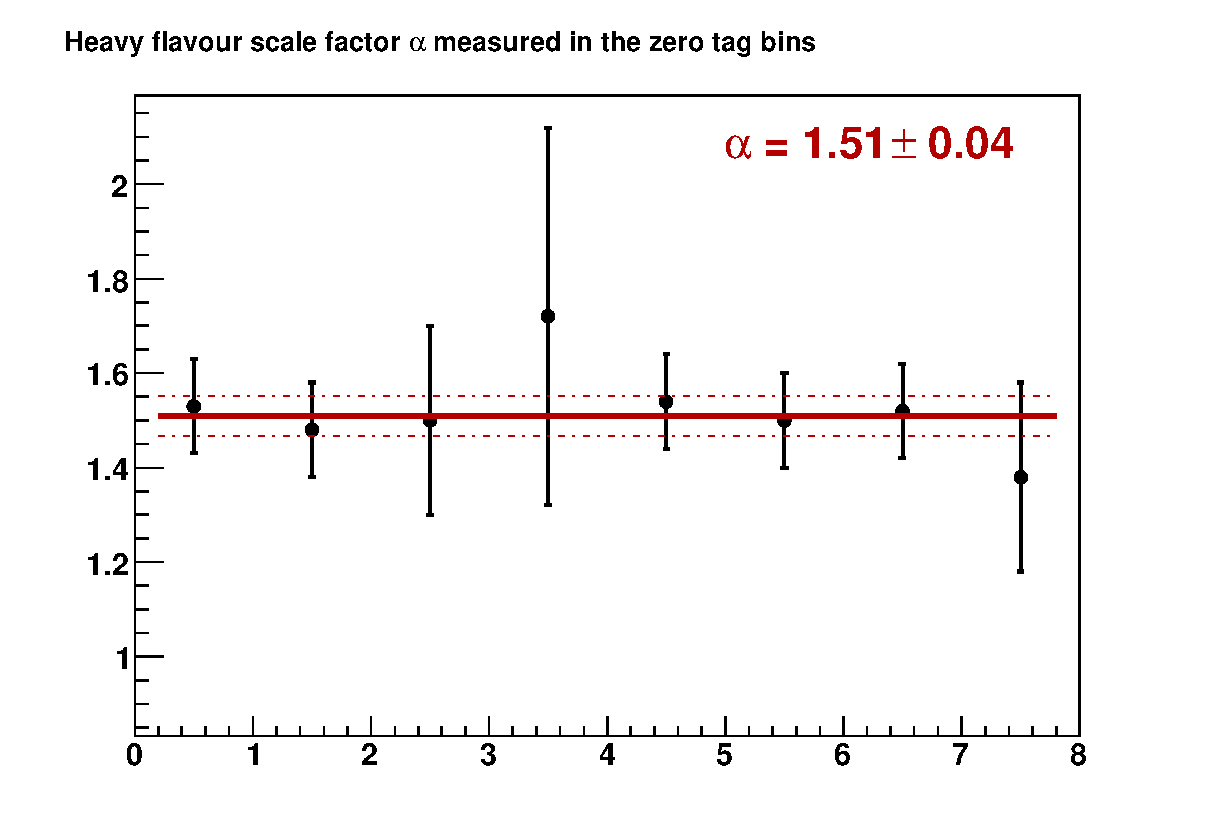
\includegraphics[width=0.75\textwidth]{eps/DataBackground/alpha.eps}
\end{center}
\vspace{-0.1in}
\caption{$\alpha$~values with errors for the eight zero $B$-tagged jet samples and the linear fit with error to the values~\cite{singletopnote}.}
\label{alphafit}
\end{figure}


\section{Background Yields}
\label{backgroundyields}

This section contains tables showing the observed number of data events, the total expected background, and the total number of expected signal events. Tables~\ref{pretag-yields},~\ref{onetag-yields}, and~\ref{twotag-yields} show the number of events for the following cases: before any $B$-jet requirement, one $B$-tagged jet, and two $B$-tagged jets.

\begin{table}[!h!tbp]
\begin{center}
\caption{Event yields after selection and before $B$ tagging.}
\label{pretag-yields}
\begin{tabular}{c|ccc|ccc}
%\multicolumn{7}{c}{\hspace{1in}\underline{Event Yields Before $B$-jet Selection}} \vspace{0.1in} \\
& \multicolumn{3}{c|}{Electron Channel} & \multicolumn{3}{c}{Muon Channel} \\
 %                        & 2 jets & 3 jets & 4 jets
    %                     & 2 jets & 3 jets & 4 jets \\
    				& 2 Jets	& 3 Jets	& 4 Jets	& 2 Jets	& 3 Jets	& 4 Jets \\
\hline
%Signals			&       	&       	&     	 	& 	 	&       	&		\\
%~~$s$-channel		&	14	&	7	&	2	&	10	&	5	&	1	\\
%~~$t$-channel		&	27	&	14	&	5	&	20	&	11	&	3	\\
%~~$tb$+$tqb$		&     14 &    41 &    21 &     6 &    2 &      9 &    31 &    16 &    5 &    1 \\
Backgrounds              &        	&       	&       	&       	&    	  	&      		\\
~~$\ttbar$			&	61	&	131	&	138	&	41	&	93	&	107	\\
%~~${\dilepton}$	&	35	&    28 	&    10 	&    27 	&    22 &    8     \\
%~~${\lepjets}$	&	26 	&   103 	&   128 	&	14 	&    71 &   99\\
~~$W$+jets		& 6,726	& 2,084	& 478	& 6,063	& 2,275	& 563	\\
%~~$Wb\bar{b}$		&	358 	&   149 	&    42 	&	312 	&   161 &   47  \\
%~~$Wc\bar{c}$		&	931	&   389 	&    93 	&	1,028 &   523 &  131 \\
%~~$Wjj$			&	5,437 & 1,546 	&   343 	&	4,723 & 1,591 &  385  \\
~~Multijets		&	1,433 &   860 	&   256 	&	329 &   223 &   58	\\
\hline
Expected Signal	& 41		& 21		& 7		& 30		& 16		& 4	\\
Background Sum    	& 8,220 	& 3,075 	&   874 	& 6,434 	& 2,592 	& 727 \\
\hline
Data                     	&	8,220 & 3,075 	&   874 	&	6,432 & 2,590 &  727 \\
\end{tabular}
\vspace{-0.1in}
\end{center}
\end{table}

\begin{table}[!h!tbp]
\begin{center}
\caption{Event yields after selection and one selected $B$-jet.}
\label{onetag-yields}
\begin{tabular}{c|ccc|ccc}
%\multicolumn{7}{c}{\hspace{1in}\underline{Event Yields with One $B$-jet}} \vspace{0.1in} \\
& \multicolumn{3}{c|}{Electron Channel} & \multicolumn{3}{c}{Muon Channel} \\
                         & 2 jets & 3 jets & 4 jets
                         & 2 jets & 3 jets & 4 jets \\
\hline
%Signals                  		&      		&      		&      		&      		&      		&      		\\
%~~$s$-channel  		&	7 	&    3		&    1 	& 5 		&    2 	&    1		\\
%~~$t$-channel 		&	11 	&    6 	&    2 	& 9 		&    5 	&    2		\\
%~~$tb$+$tqb$             	&	18 	&    9 	&    3 	& 14 		&    7		 &    2	\\
Backgrounds              	&      		&      	 	&      		&      		&      		&      		\\
~~$\ttbar$				&	27	&	60	&	63	&	19	&	42	&	49	\\
%~~${\dilepton}$     		&	16 	&   13 	&    5 	& 13 		&   10 	&    4		\\
%~~${\lepjets}$		 	&	11 	&   47 	&   58 	& 6 		&   32 	&   45	\\
~~$W$+jets			&	255	&	106	&	28	&	242	&	125	&	35	\\
%~~$Wb\bar{b}$            	&	120 	&   50 	&   14 	& 110 	&   56 	&   16	\\
%~~$Wc\bar{c}$            	&	74 	&   36 	&    9 	& 74 		&   46 	&   13	\\
%~~$Wjj$                  		&	61 	&   20 	&    5 	& 58 		&   23 	&    6		\\
~~Multijets              		&	66 	&   48 	&   18 	& 26 		&   24 	&    8		\\
\hline                                                                            
Expected Signal		& 	18	&	9	&	3	&	14	&	7	& 2		\\
Background Sum           	&  	348	&  213 	&  110 	& 286 	&  191 	&   93	\\
\hline                                                                            
Data                     		&  	357 	&  207 	&   97 	&	287 	&  179 	&  100
\end{tabular}
\vspace{-0.1in}
\end{center}
\end{table}

\begin{table}[!h!tbp]
\begin{center}
\caption{Event yields after selection and two selected $B$-jets.}
\label{twotag-yields}
\begin{tabular}{c|ccc|ccc}
%\multicolumn{7}{c}{\hspace{1in}\underline{Event Yields with Two $B$-jets}} \vspace{0.1in} \\
& \multicolumn{3}{c|}{Electron Channel} & \multicolumn{3}{c}{Muon Channel} \\
                         & 2 jets & 3 jets & 4 jets
                         & 2 jets & 3 jets & 4 jets	\\
\hline
%Signals                  	&      		&      		&       	&       	&       	&       	\\
%~~$s$-channel     	&	2.3 	&   1.1 	&   0.3 	& 1.9 	&   0.9 	&   0.3	\\
%~~$t$-channel    	&	0.3 	&   0.8 	&   0.4 	&  0.2 	&   0.7 	&   0.4	\\
%~~$tb$+$tqb$          	&	2.6 	&   1.9 	&   0.7 	&  2.1 	&   1.6 	&   0.6	\\
Backgrounds            	&		&      		&       	&       	&       	&       	\\
~~$\ttbar$			&	7.2	&	18.2	&	23.5	&	5.6	&	15.0	&	19.4	\\
%~~${\dilepton}$     	&	5.5 	&   4.6 	&   1.7 	&  4.6 	&   3.8 	&   1.4	\\
%~~${\lepjets}$ 		&	1.7 	&  13.6 	&  21.8 	& 1.0 	&  10.2 	&  18.0	\\
~~$W$+jets		&	17.9	&	8.0	&	2.2	&	17.0	&	9.8	&	2.8	\\
%~~$Wb\bar{b}$        	&	16.2 &   6.8 	&   1.8 	& 15.3 	&   8.2 	&   2.3	\\
%~~$Wc\bar{c}$         	&	1.6 	&   1.1 	&   0.4 	& 1.6 	&   1.5 	&   0.5	\\
%~~$Wjj$                  	&	0.1 	&   0.1 	&   0.0 	& 0.1 	&   0.1 	&   0.0	\\
~~Multijets              	&  	2.5 	&   3.2 	&   2.7 	& 1.5 	&   1.9 	&   0.4	\\
\hline                                                                                       
Expected Signal	& 	2.6	&	1.9	&	0.7	&	2.1	&	1.6	& 0.6		\\
Background Sum   	&	27.5	&	29.4 	&	28.4	&	24.1	&  25.7 	&  22.7	\\
\hline                                                                                       
Data                     	&	30	&   37  	&   22  	&	23  	&   32  	&   27  
\end{tabular}
\vspace{-0.1in}
\end{center}
\end{table}

\clearpage
\section{Comparison of Data with Expection}
\label{databackcompare}

The following histograms compare data with the sum of the expected background for events before $B$-tagging, events with one $B$-tag, and events with two $B$-tags. Four kinematic variables are shown: leading jet p$_{T}$ (jet with largest p$_{T}$), second jet p$_{T}$ (jet with second largest p$_{T}$), lepton p$_{T}$ (either electron or muon), and missing E$_{T}$. The error bands on the plots represent the combined statistical and systematic error for the data sample. A description and magnitude of each systematic error can be found in Chapter~\ref{limits}. All plots show combined electron and muon events.

All histograms use the same color convention for backgrounds. The convention is shown in Fig.~\ref{convention}.


\begin{figure}[!h!tbp]
\begin{center}
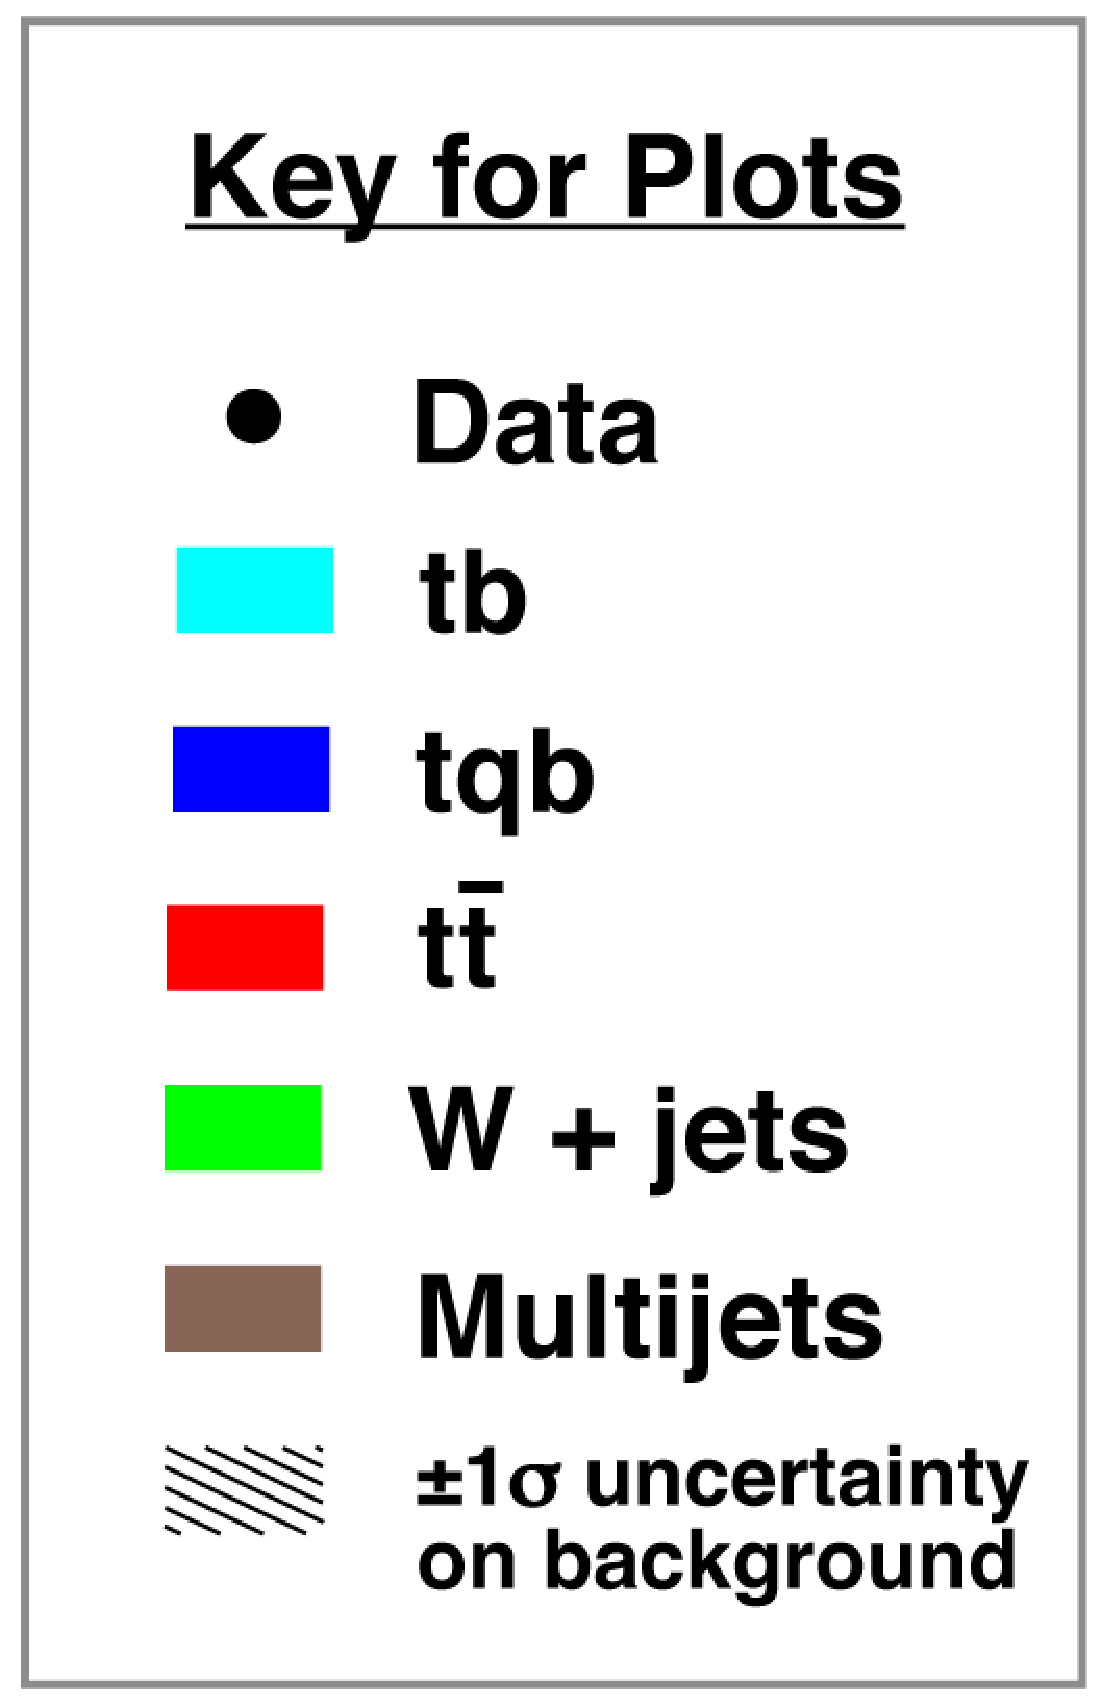
\includegraphics[width=0.42\textwidth]{eps/DataBackground/plot_key.eps}
\end{center}
\vspace{-0.1in}
\caption{Color convention used in all histograms.}
\label{convention}
\end{figure}

\clearpage
\begin{center}
LEADING JET P$_{T}$
\end{center}

\begin{figure}[!h!tbp]
\begin{center}
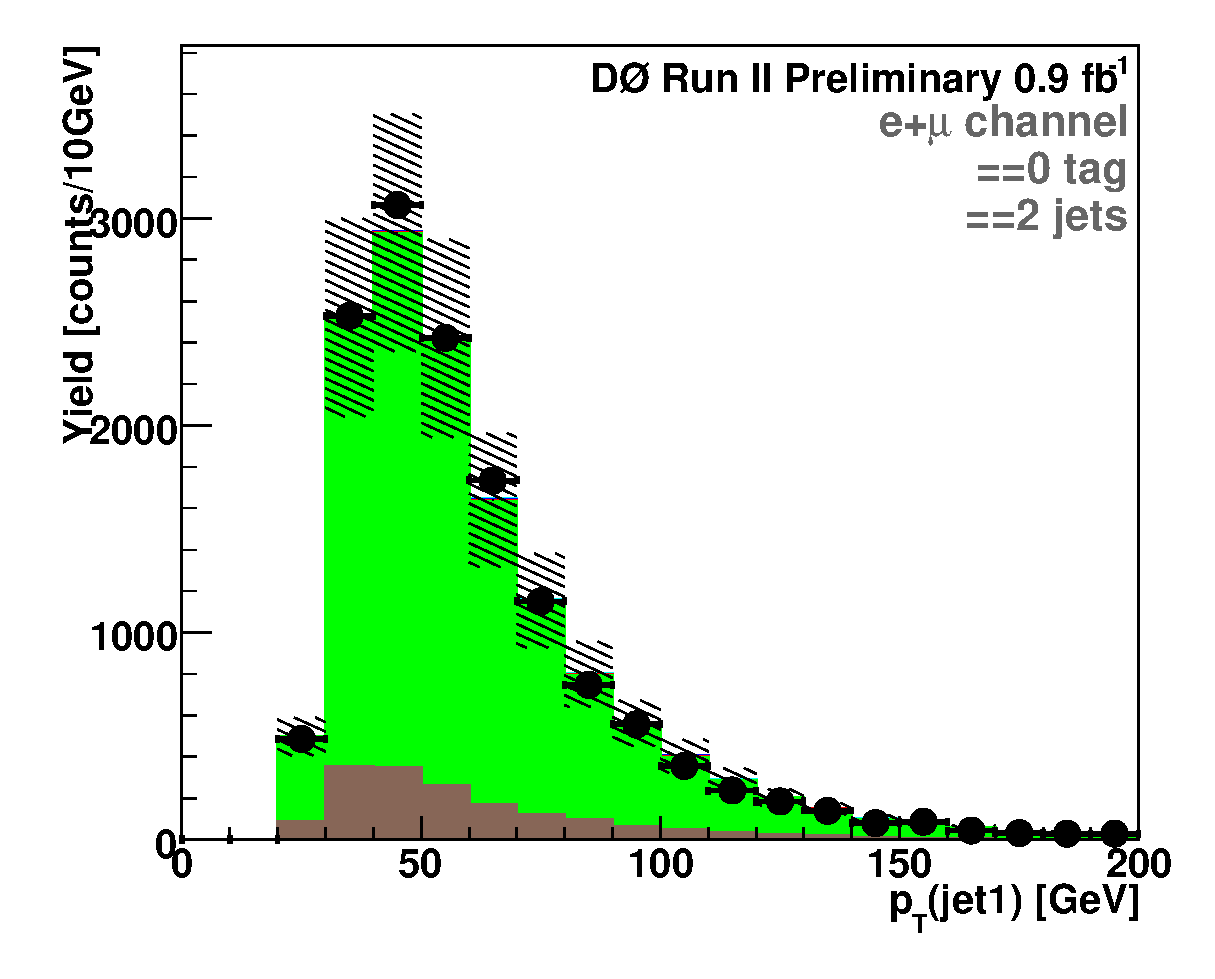
\includegraphics[width=0.32\textwidth]{eps/DataBackground/EMU/emu_EqZeroTag_EqTwoJet_Jet1Pt.eps}
\includegraphics[width=0.32\textwidth]{eps/DataBackground/EMU/emu_EqOneTag_EqTwoJet_Jet1Pt.eps}
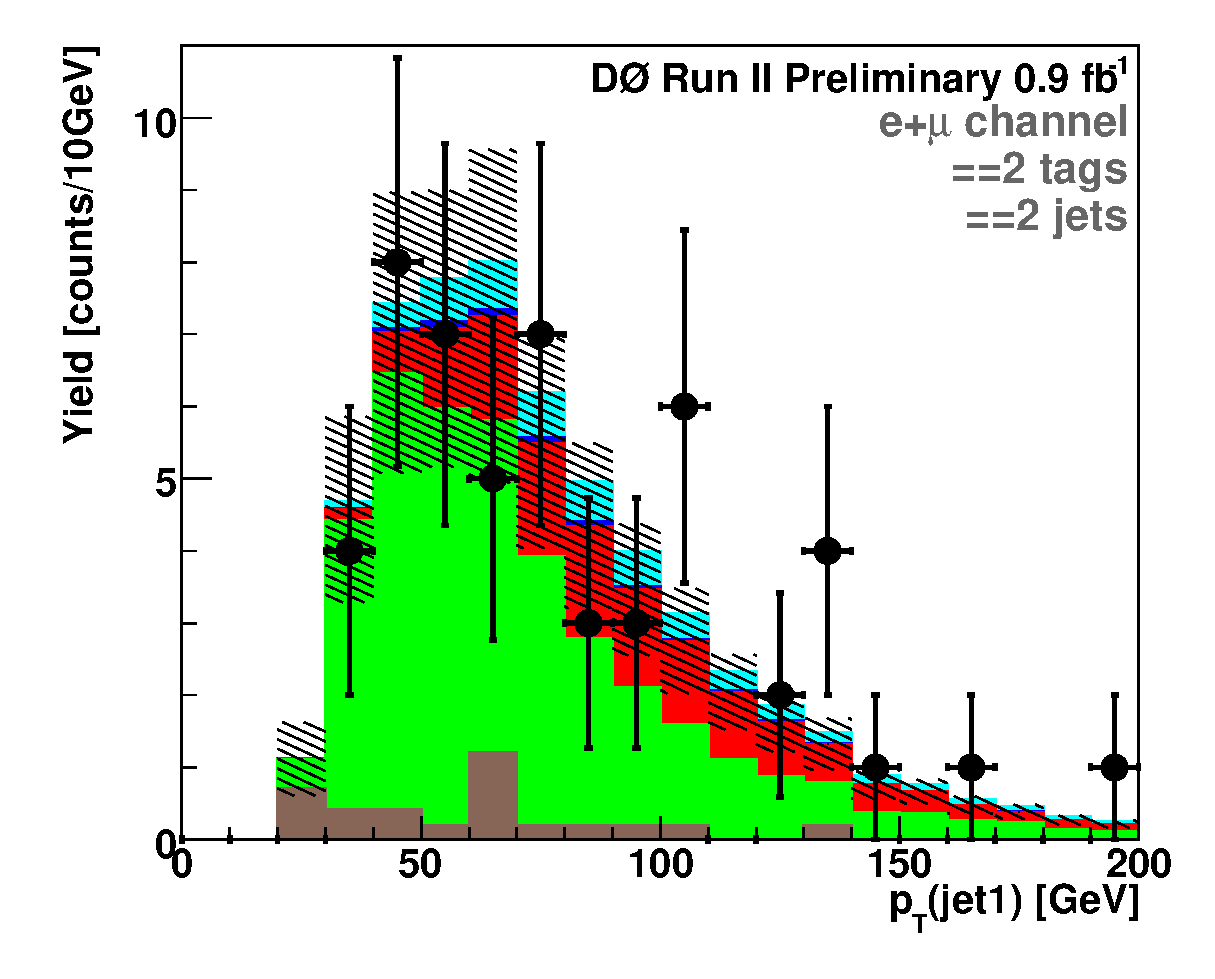
\includegraphics[width=0.32\textwidth]{eps/DataBackground/EMU/emu_EqTwoTag_EqTwoJet_Jet1Pt.eps}
\includegraphics[width=0.32\textwidth]{eps/DataBackground/EMU/emu_EqZeroTag_EqThreeJet_Jet1Pt.eps}
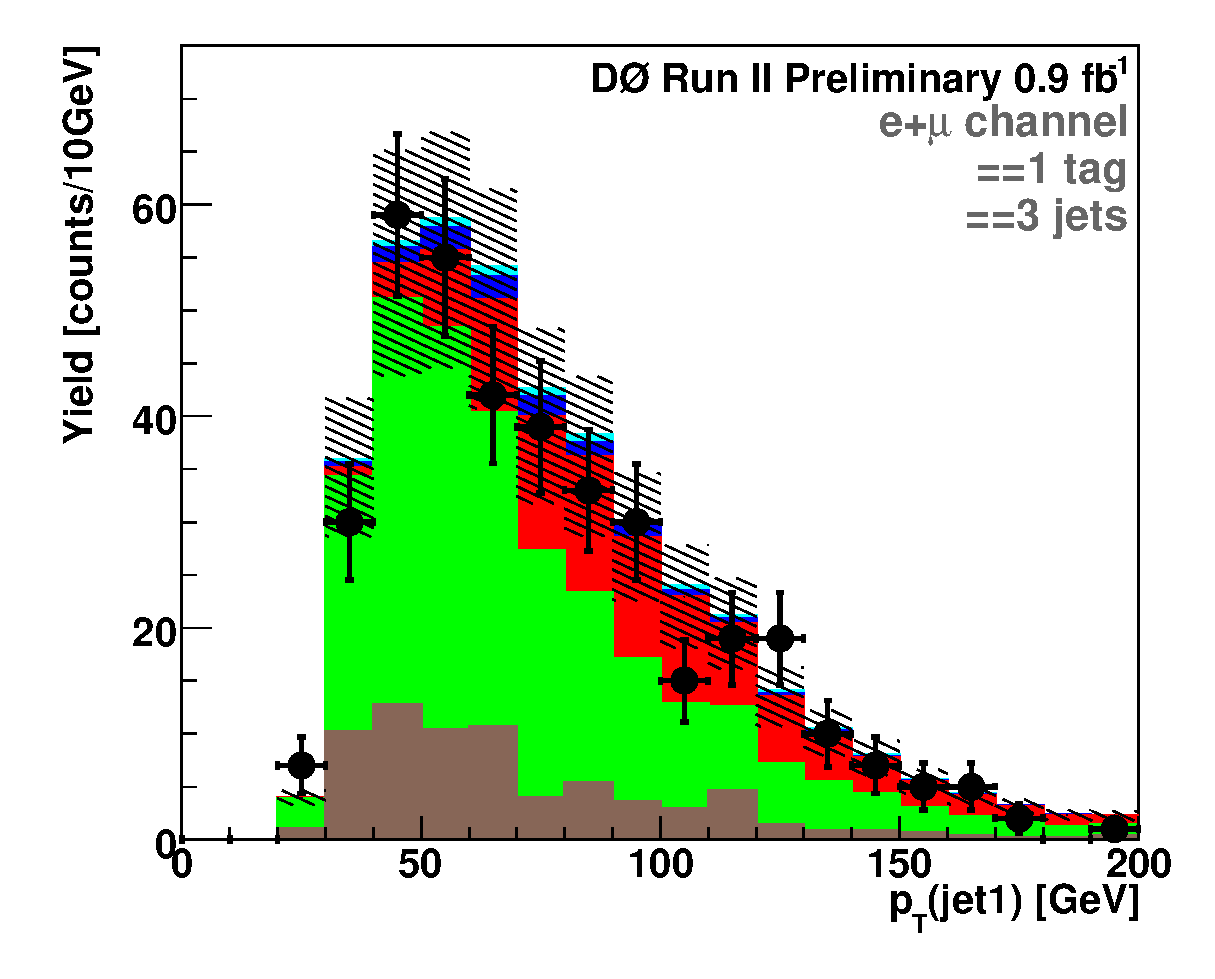
\includegraphics[width=0.32\textwidth]{eps/DataBackground/EMU/emu_EqOneTag_EqThreeJet_Jet1Pt.eps}
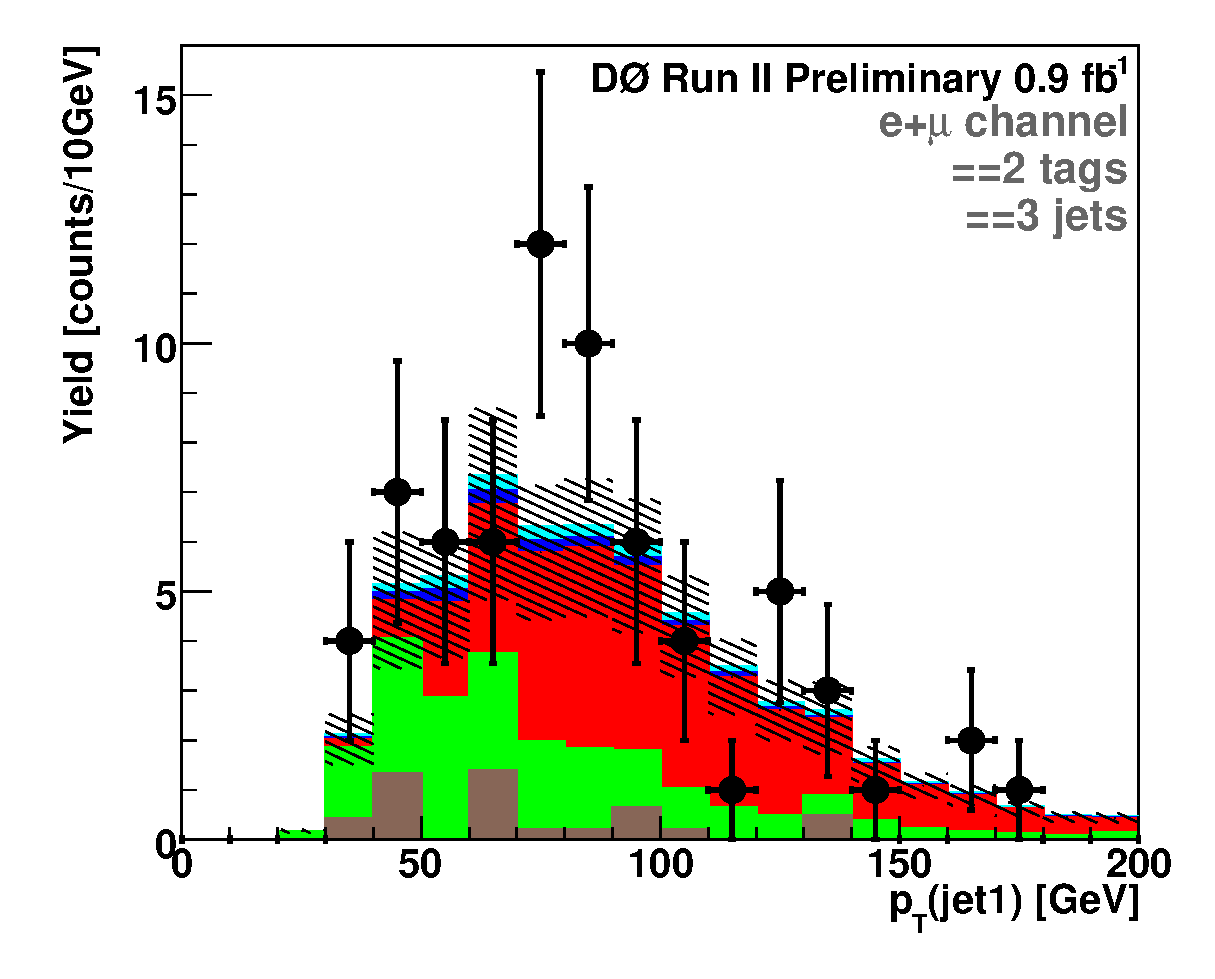
\includegraphics[width=0.32\textwidth]{eps/DataBackground/EMU/emu_EqTwoTag_EqThreeJet_Jet1Pt.eps}
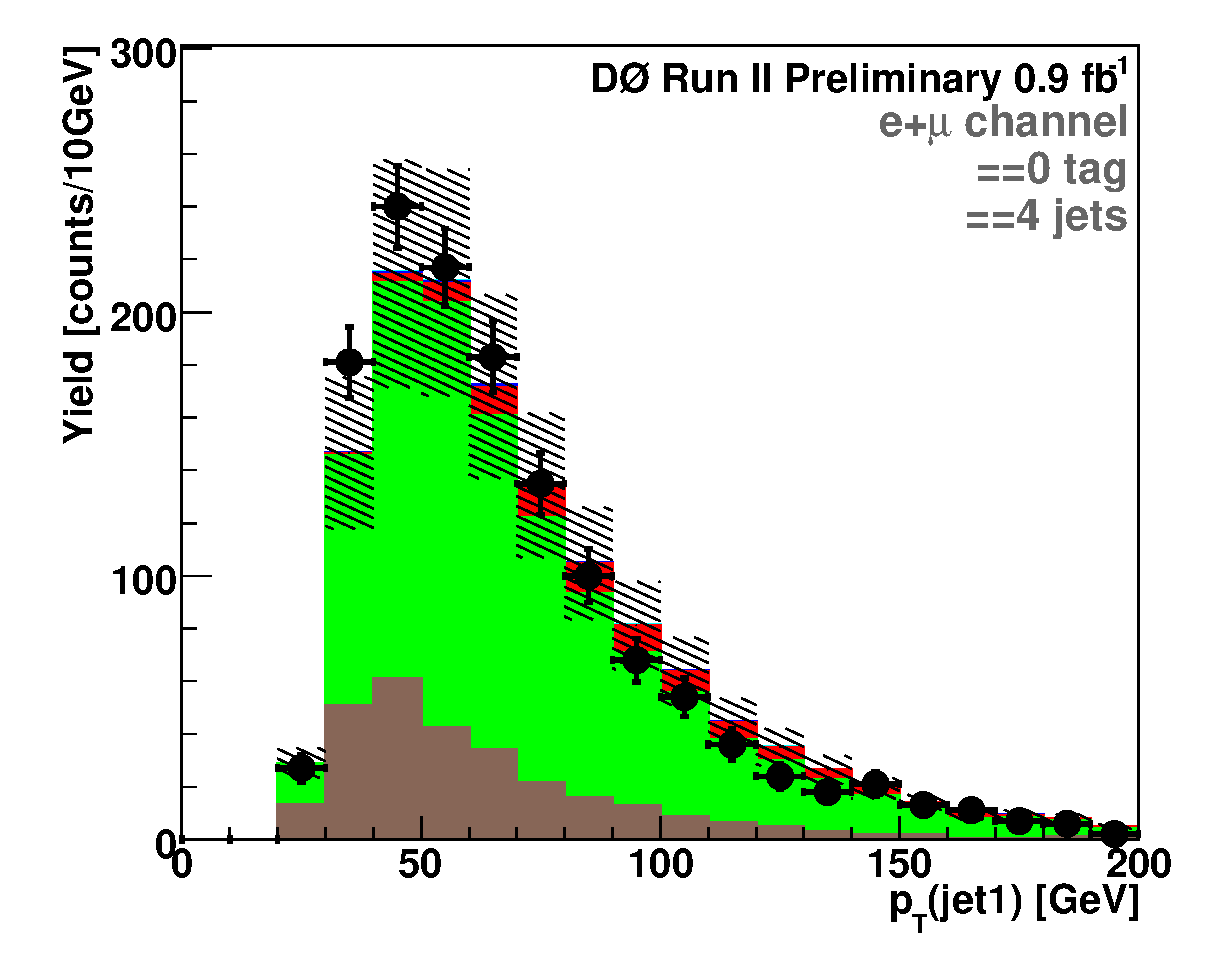
\includegraphics[width=0.32\textwidth]{eps/DataBackground/EMU/emu_EqZeroTag_EqFourJet_Jet1Pt.eps}
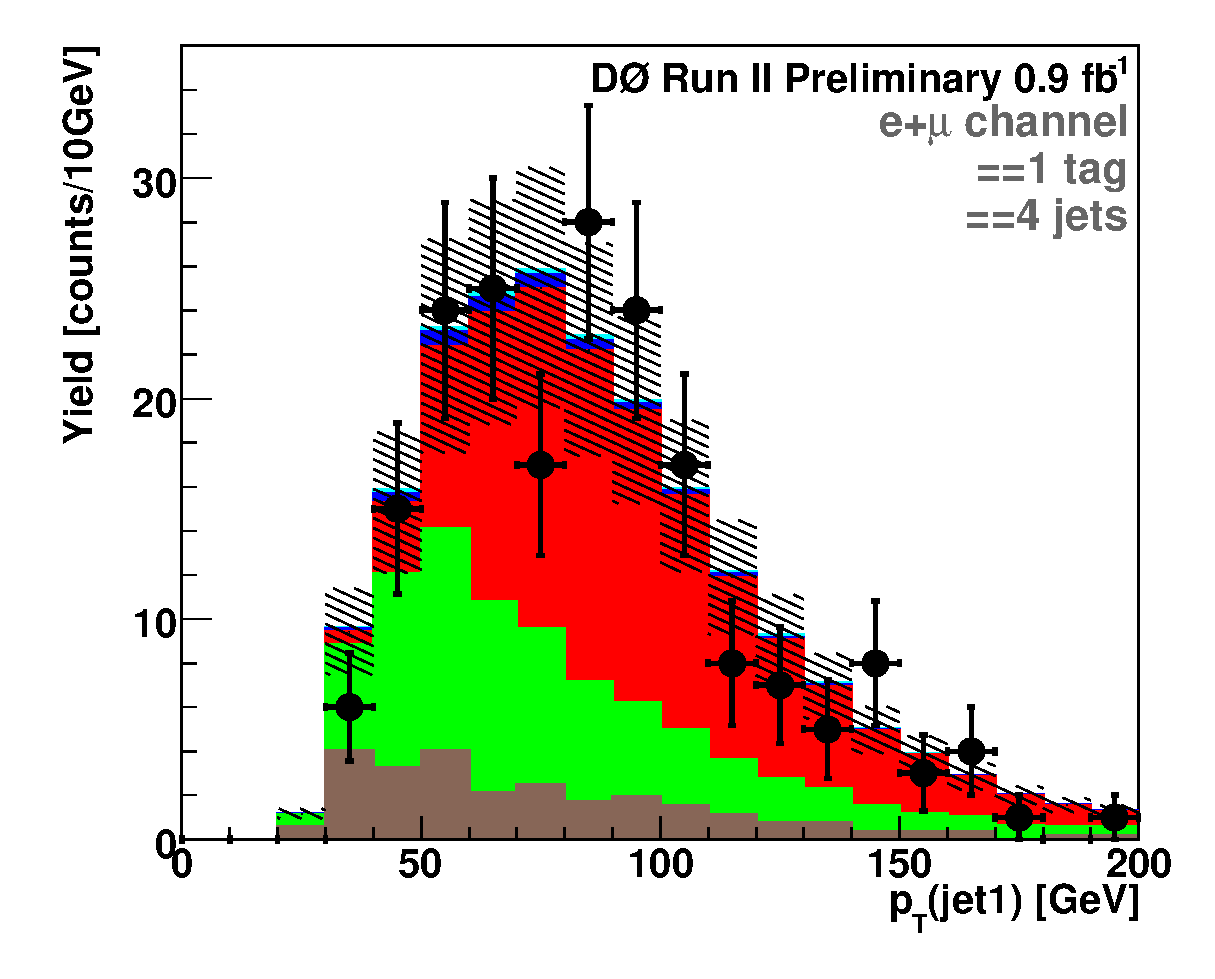
\includegraphics[width=0.32\textwidth]{eps/DataBackground/EMU/emu_EqOneTag_EqFourJet_Jet1Pt.eps}
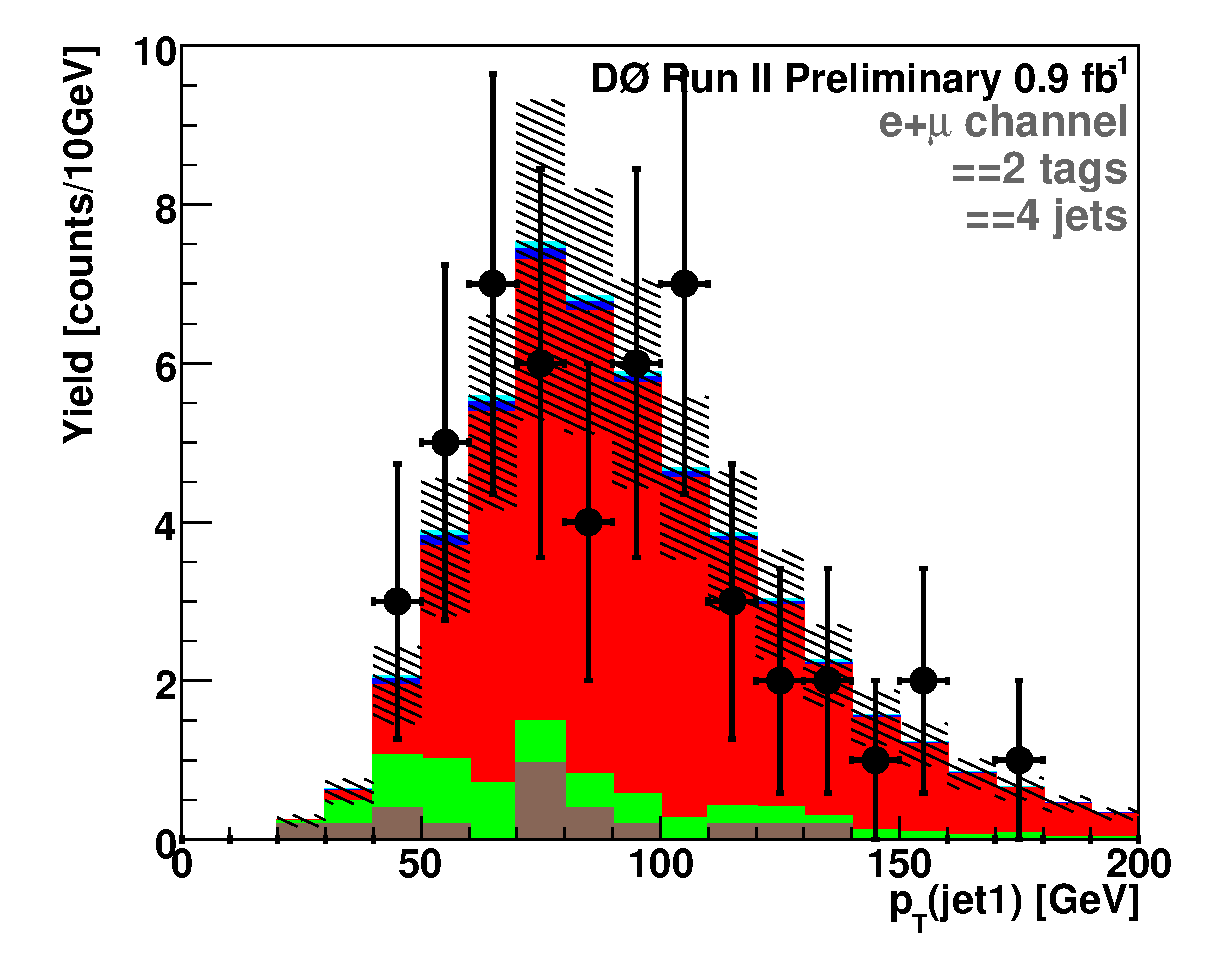
\includegraphics[width=0.32\textwidth]{eps/DataBackground/EMU/emu_EqTwoTag_EqFourJet_Jet1Pt.eps}
\end{center}
\vspace{-0.1in}
\caption{Leading jet p$_{T}$ distributions. Upper row: events with 2 jets, Middle row: events with 3 jets, Lower row: events with 4 jets. Left column: events before $B$-tagging, Middle row: events with one selected $B$-jet, Right column: events with two selected $B$-jets~\cite{singletopnote}.}
\label{Jet1pt}
\end{figure}



\clearpage
\begin{center}
SECOND JET P$_{T}$
\end{center}

\begin{figure}[!h!tbp]
\begin{center}
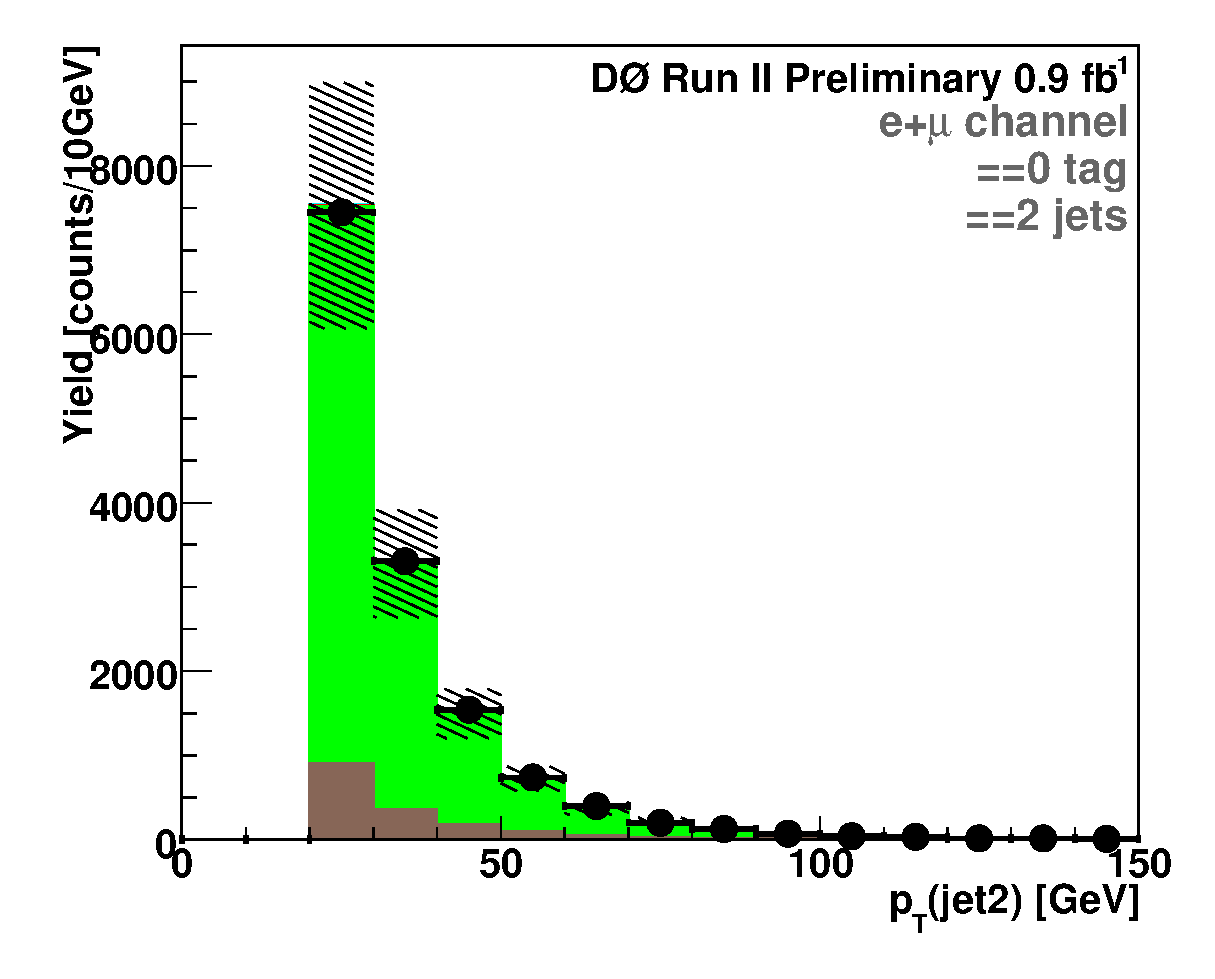
\includegraphics[width=0.32\textwidth]{eps/DataBackground/EMU/emu_EqZeroTag_EqTwoJet_Jet2Pt.eps}
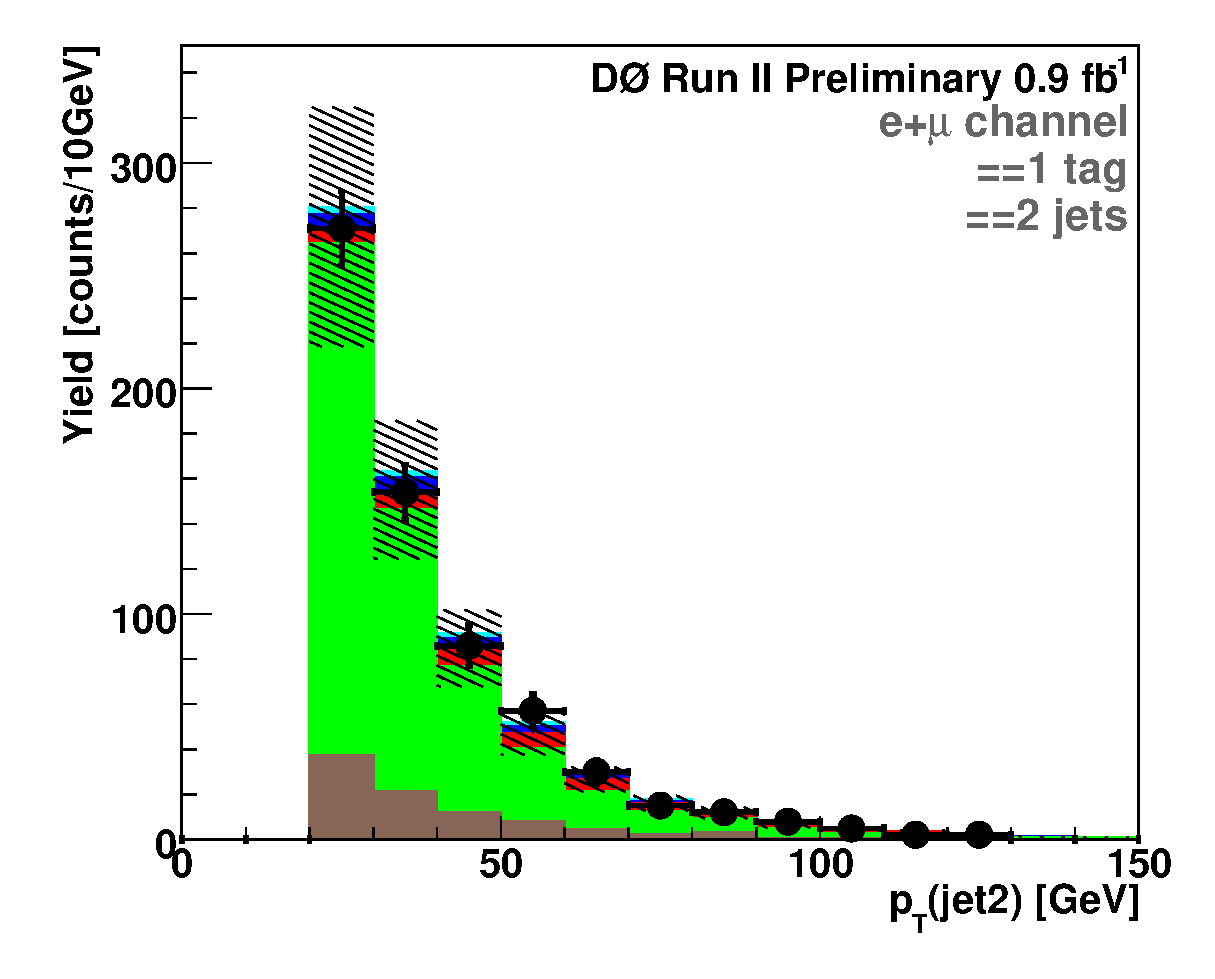
\includegraphics[width=0.32\textwidth]{eps/DataBackground/EMU/emu_EqOneTag_EqTwoJet_Jet2Pt.eps}
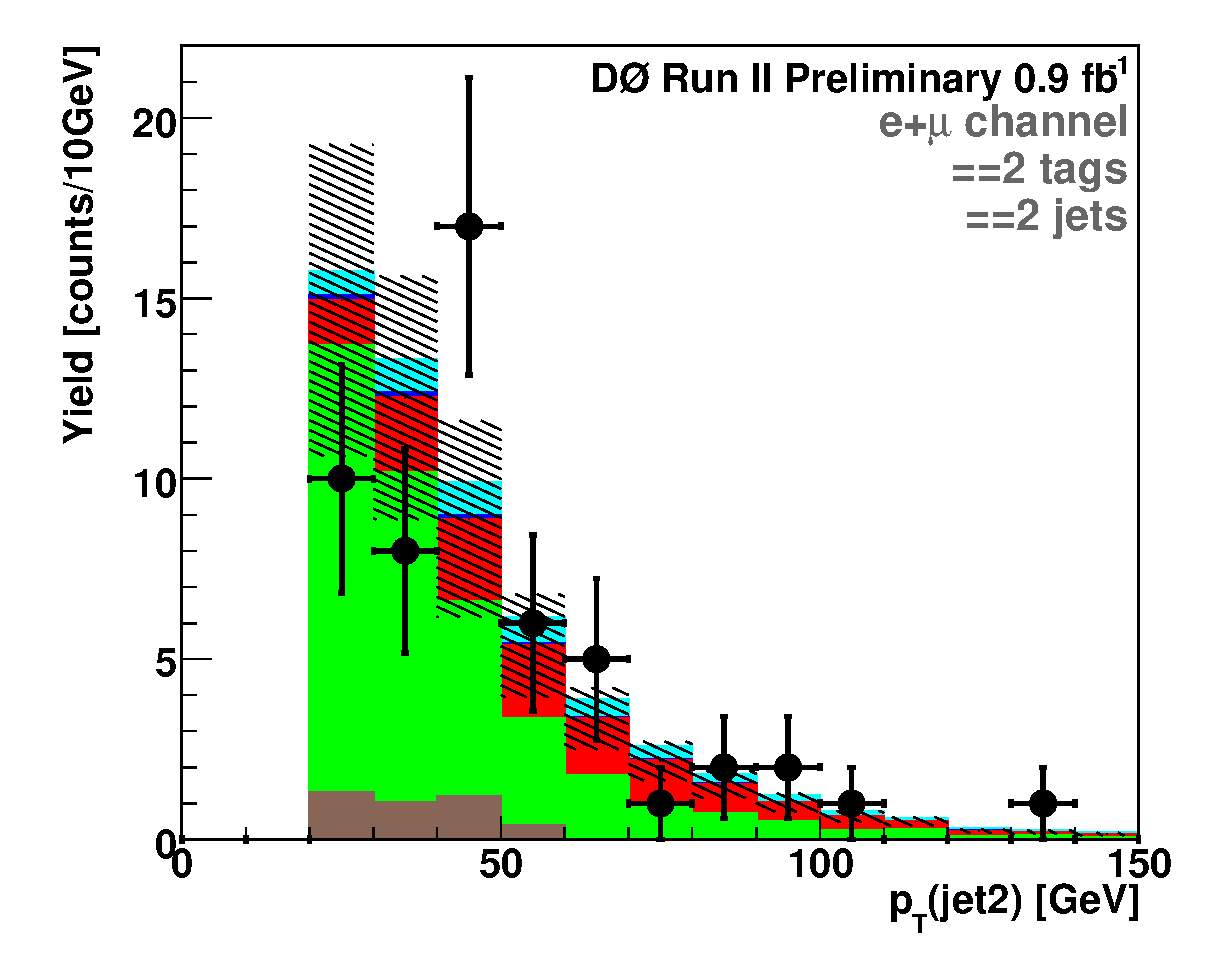
\includegraphics[width=0.32\textwidth]{eps/DataBackground/EMU/emu_EqTwoTag_EqTwoJet_Jet2Pt.eps}
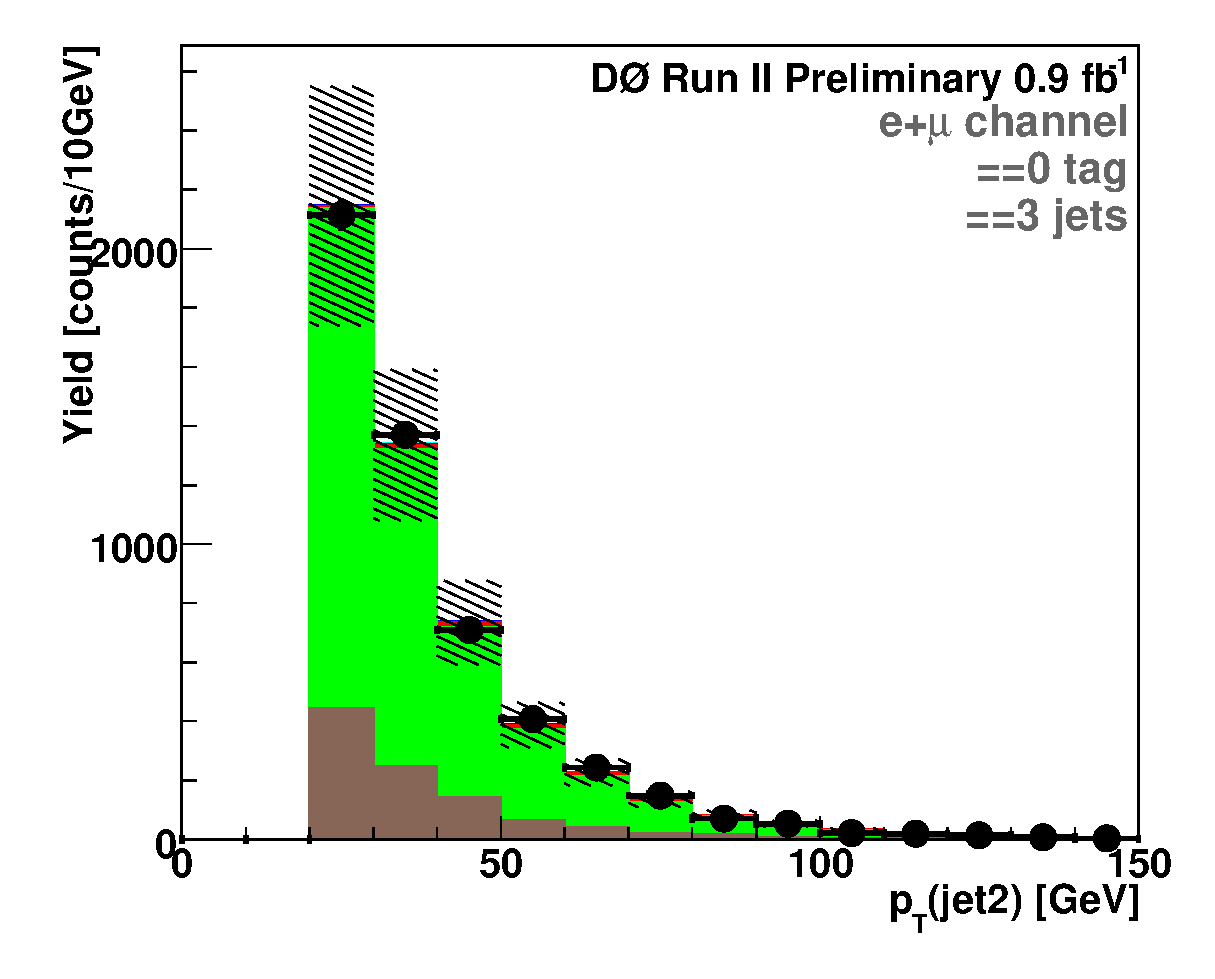
\includegraphics[width=0.32\textwidth]{eps/DataBackground/EMU/emu_EqZeroTag_EqThreeJet_Jet2Pt.eps}
\includegraphics[width=0.32\textwidth]{eps/DataBackground/EMU/emu_EqOneTag_EqThreeJet_Jet2Pt.eps}
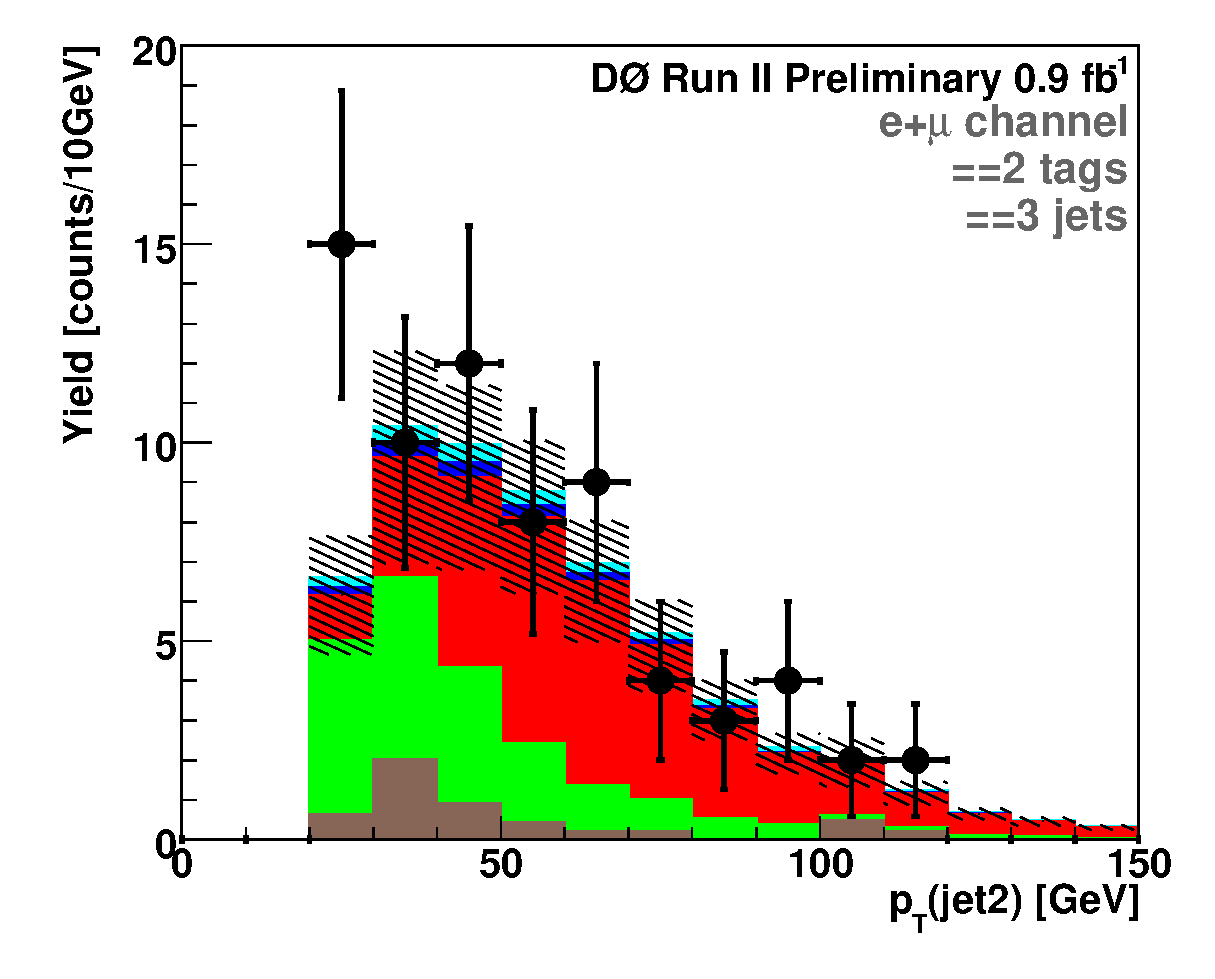
\includegraphics[width=0.32\textwidth]{eps/DataBackground/EMU/emu_EqTwoTag_EqThreeJet_Jet2Pt.eps}
\includegraphics[width=0.32\textwidth]{eps/DataBackground/EMU/emu_EqZeroTag_EqFourJet_Jet2Pt.eps}
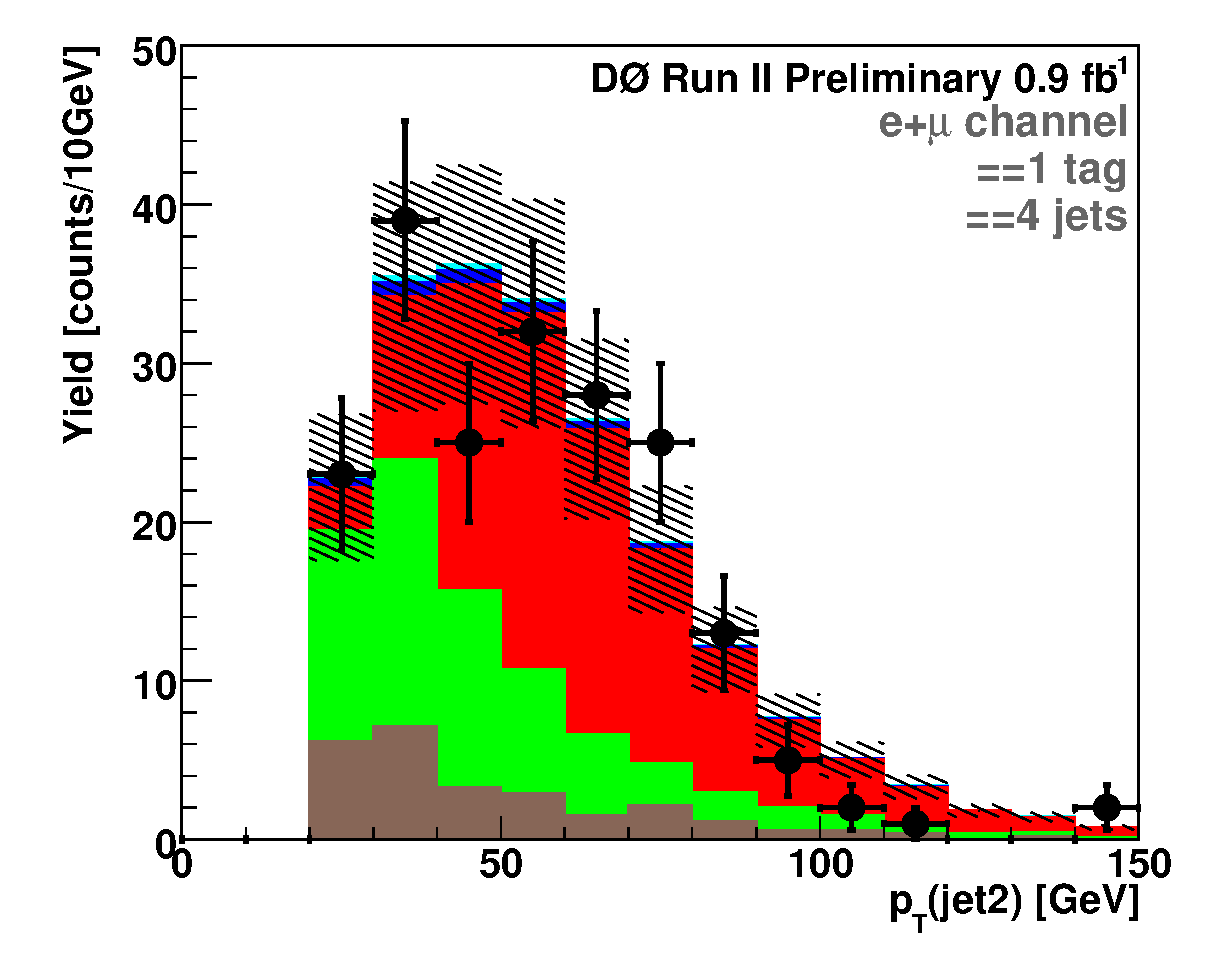
\includegraphics[width=0.32\textwidth]{eps/DataBackground/EMU/emu_EqOneTag_EqFourJet_Jet2Pt.eps}
\includegraphics[width=0.32\textwidth]{eps/DataBackground/EMU/emu_EqTwoTag_EqFourJet_Jet2Pt.eps}
\end{center}
\vspace{-0.1in}
\caption{Second leading jet p$_{T}$ distributions. Upper row: events with 2 jets, Middle row: events with 3 jets, Lower row: events with 4 jets. Left column: events before $B$-tagging, Middle row: events with one selected $B$-jet, Right column: events with two selected $B$-jets~\cite{singletopnote}.}
\label{Jet2pt}
\end{figure}




\clearpage
\begin{center}
LEPTON P$_{T}$
\end{center}

\begin{figure}[!h!tbp]
\begin{center}
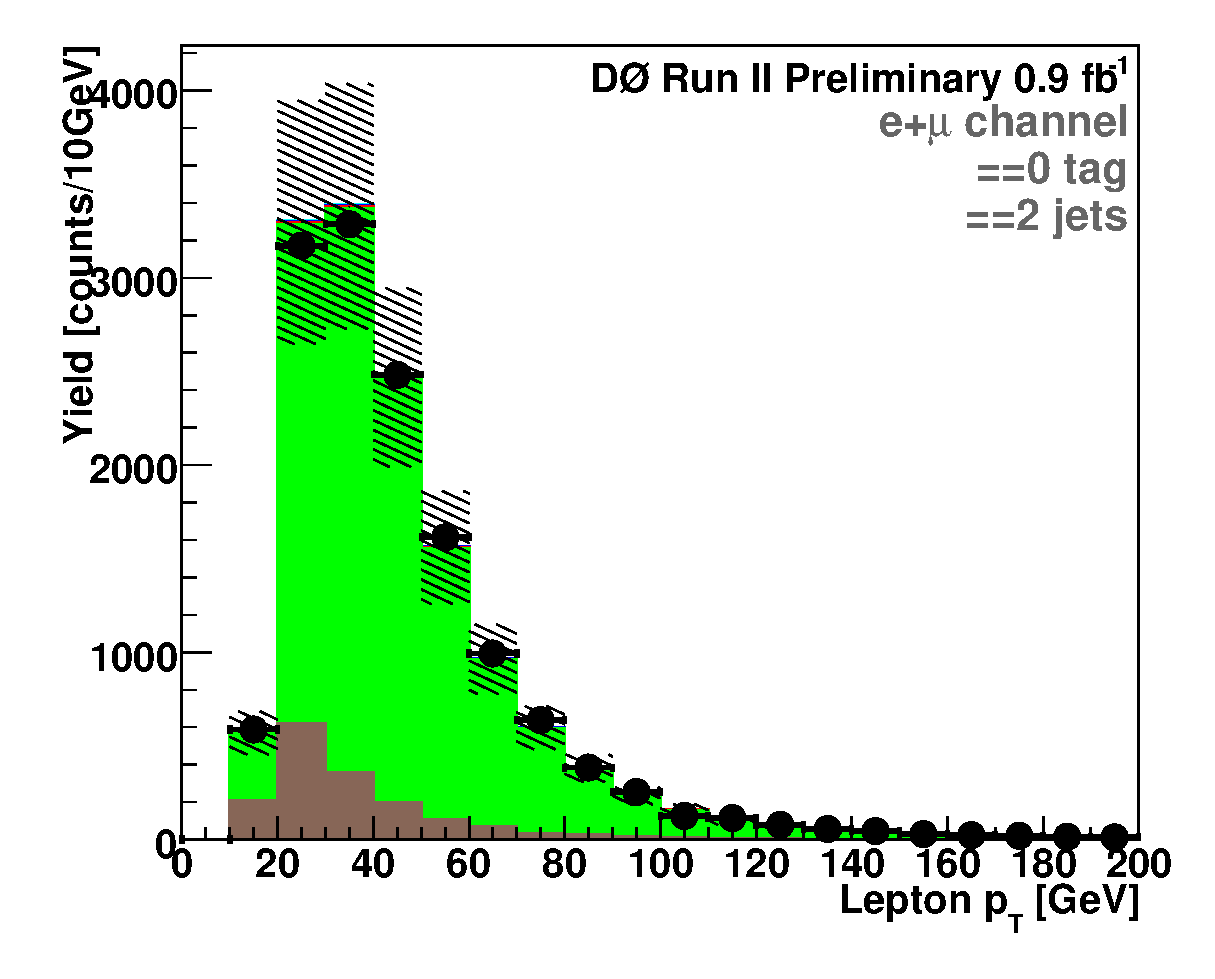
\includegraphics[width=0.32\textwidth]{eps/DataBackground/EMU/emu_EqZeroTag_EqTwoJet_LeptonPt.eps}
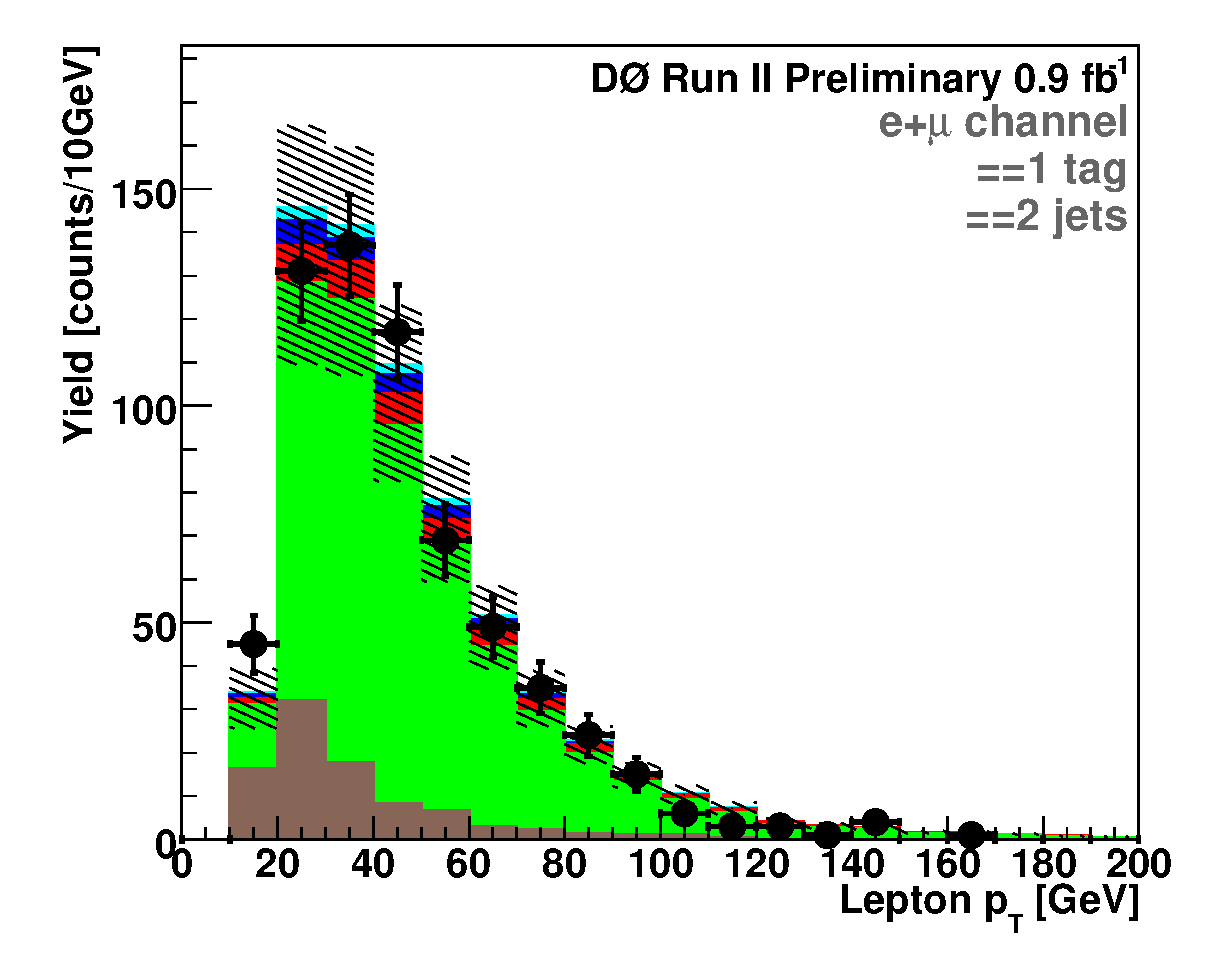
\includegraphics[width=0.32\textwidth]{eps/DataBackground/EMU/emu_EqOneTag_EqTwoJet_LeptonPt.eps}
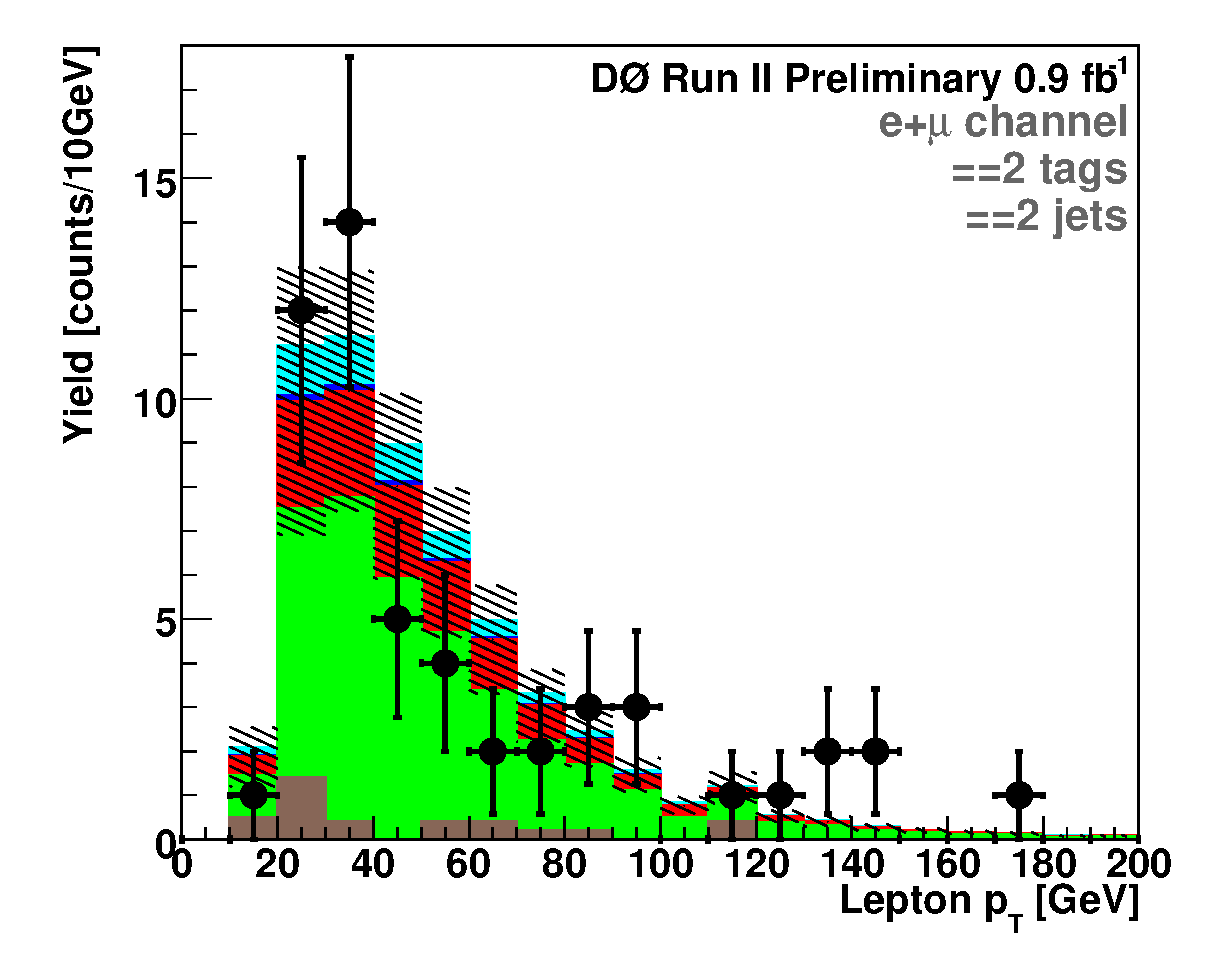
\includegraphics[width=0.32\textwidth]{eps/DataBackground/EMU/emu_EqTwoTag_EqTwoJet_LeptonPt.eps}
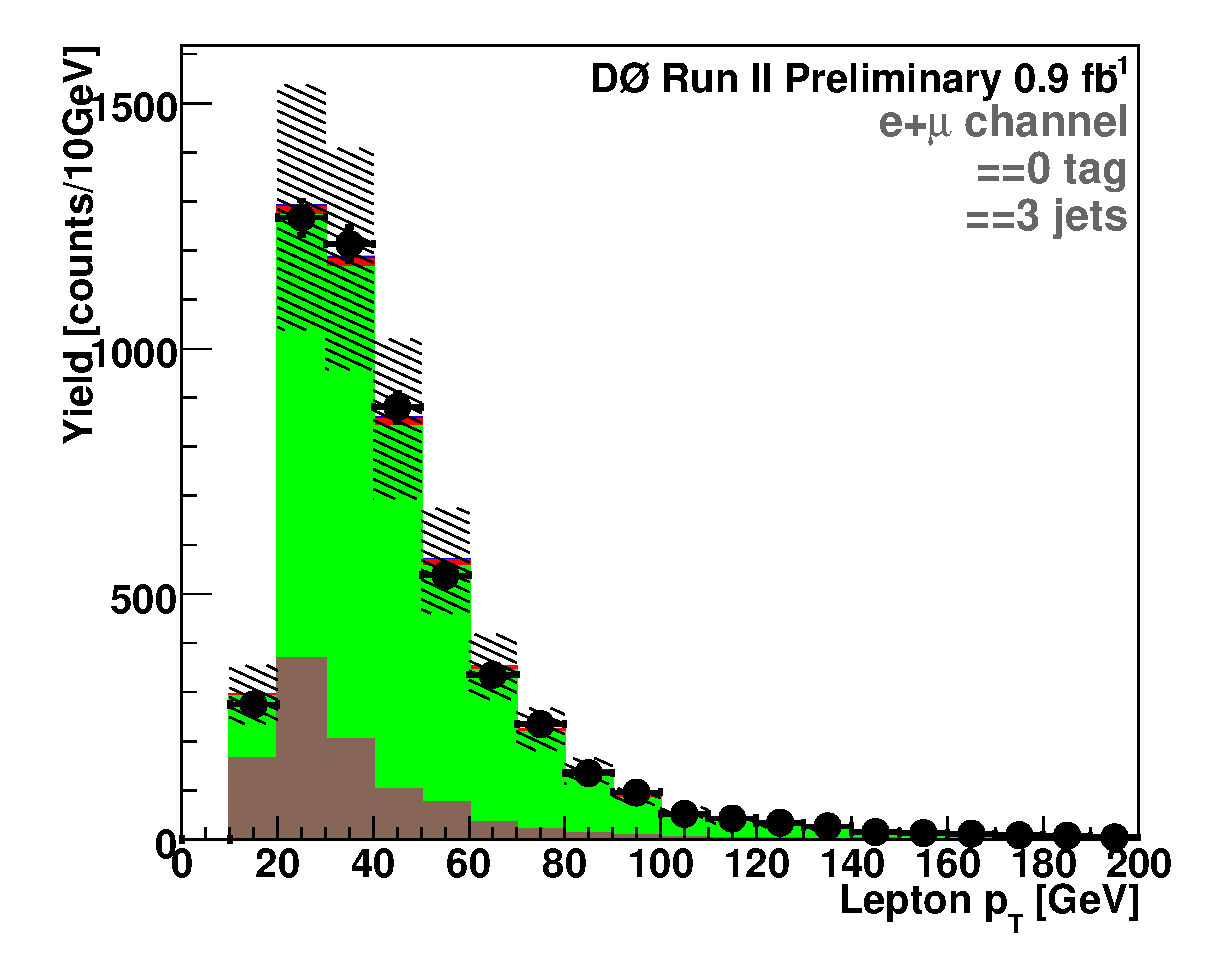
\includegraphics[width=0.32\textwidth]{eps/DataBackground/EMU/emu_EqZeroTag_EqThreeJet_LeptonPt.eps}
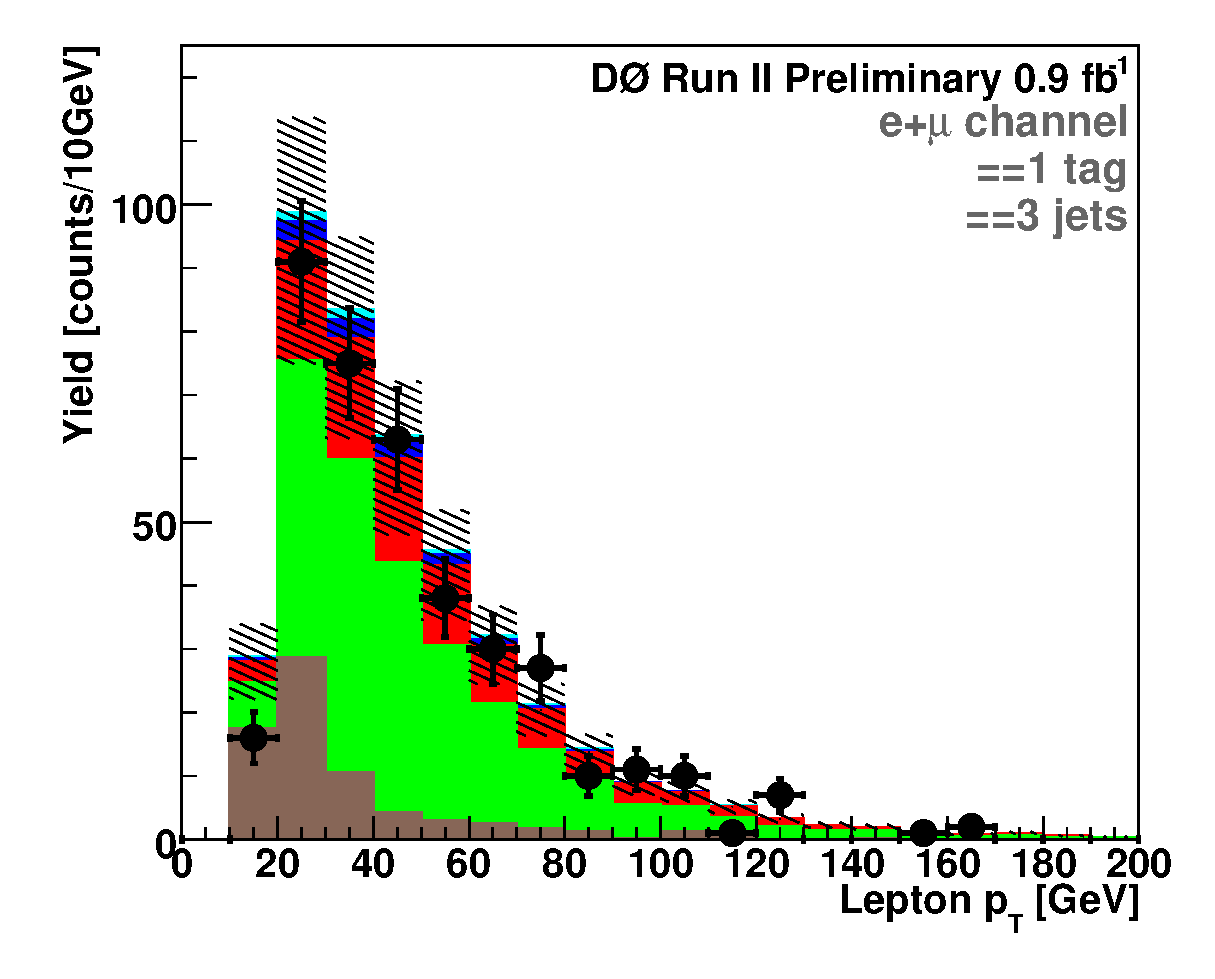
\includegraphics[width=0.32\textwidth]{eps/DataBackground/EMU/emu_EqOneTag_EqThreeJet_LeptonPt.eps}
\includegraphics[width=0.32\textwidth]{eps/DataBackground/EMU/emu_EqTwoTag_EqThreeJet_LeptonPt.eps}
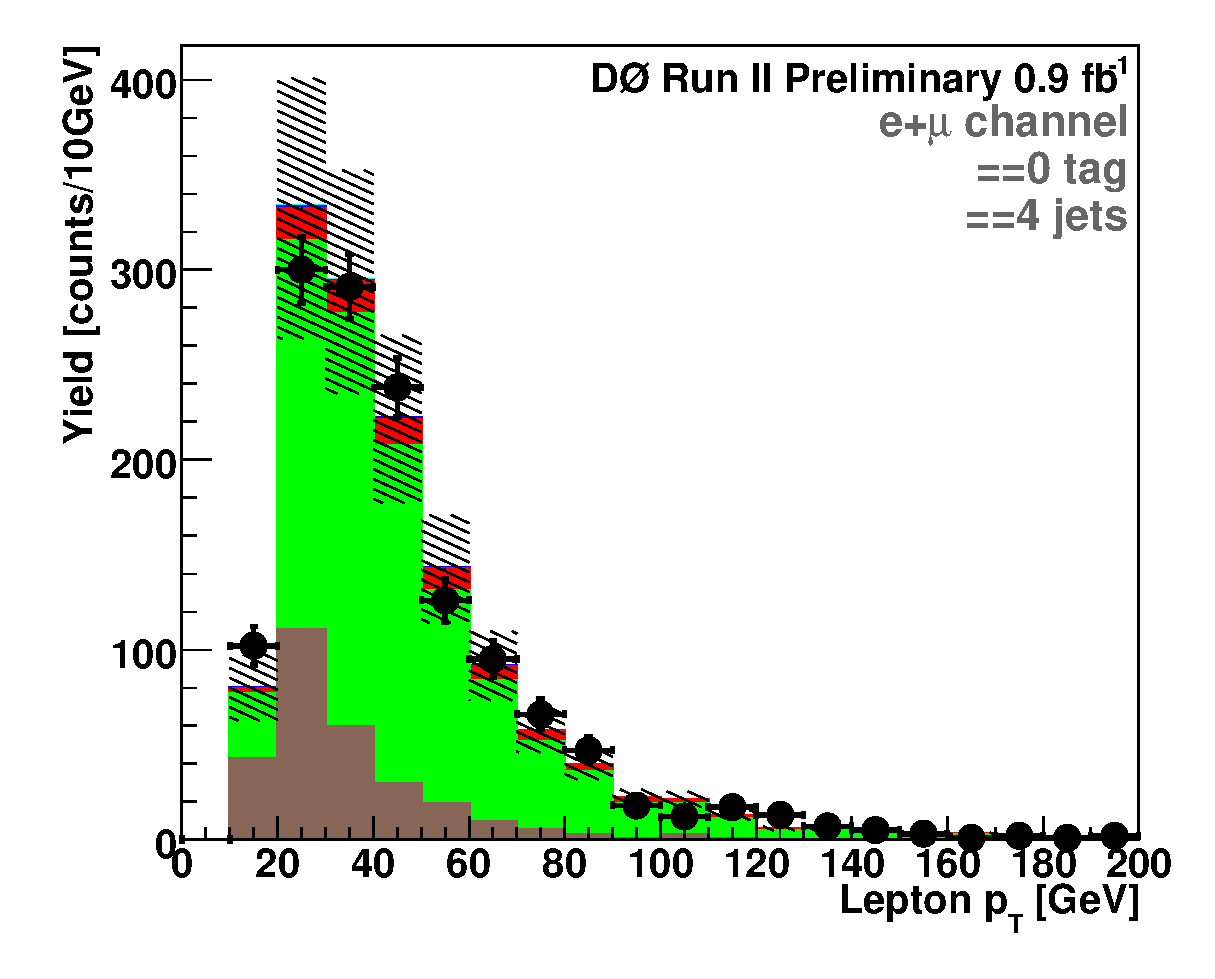
\includegraphics[width=0.32\textwidth]{eps/DataBackground/EMU/emu_EqZeroTag_EqFourJet_LeptonPt.eps}
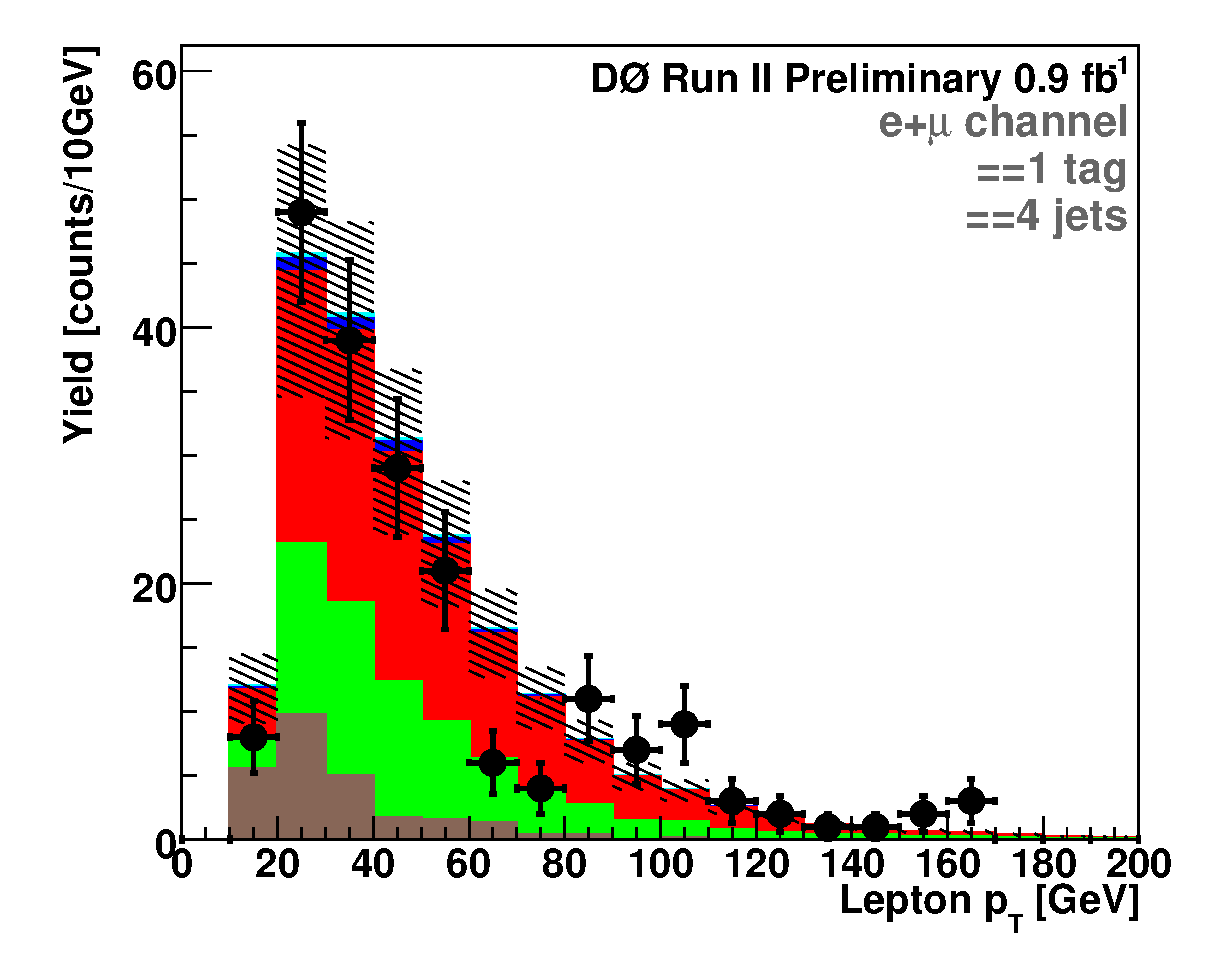
\includegraphics[width=0.32\textwidth]{eps/DataBackground/EMU/emu_EqOneTag_EqFourJet_LeptonPt.eps}
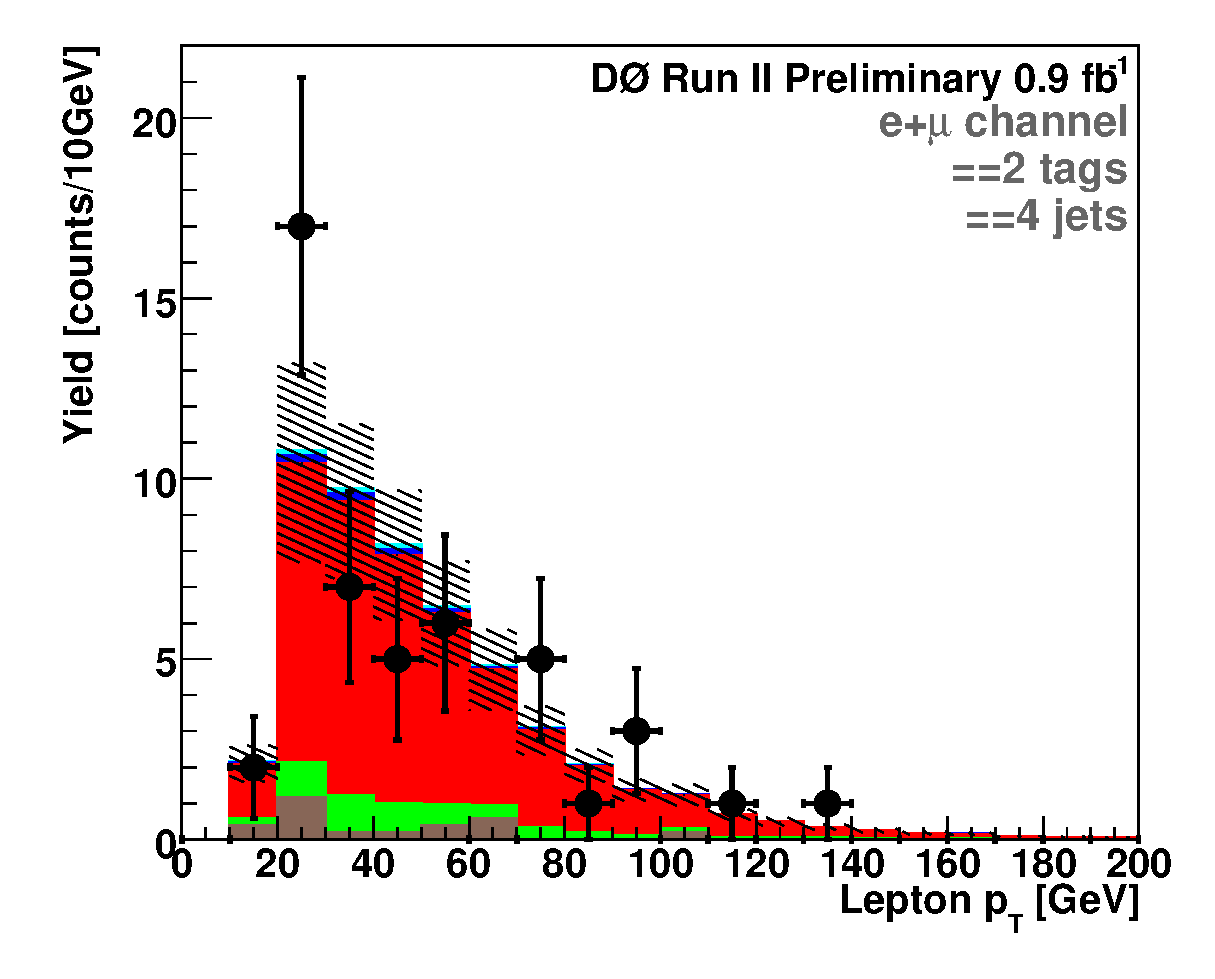
\includegraphics[width=0.32\textwidth]{eps/DataBackground/EMU/emu_EqTwoTag_EqFourJet_LeptonPt.eps}
\end{center}
\vspace{-0.1in}
\caption{Lepton p$_{T}$ distributions. Upper row: events with 2 jets, Middle row: events with 3 jets, Lower row: events with 4 jets. Left column: events before $B$-tagging, Middle row: events with one selected $B$-jet, Right column: events with two selected $B$-jets~\cite{singletopnote}.}
\label{Leptonpt}
\end{figure}




\clearpage
\begin{center}
MISSING E$_{T}$
\end{center}

\begin{figure}[!h!tbp]
\begin{center}
\includegraphics[width=0.32\textwidth]{eps/DataBackground/EMU/emu_EqZeroTag_EqTwoJet_MissingEt.eps}
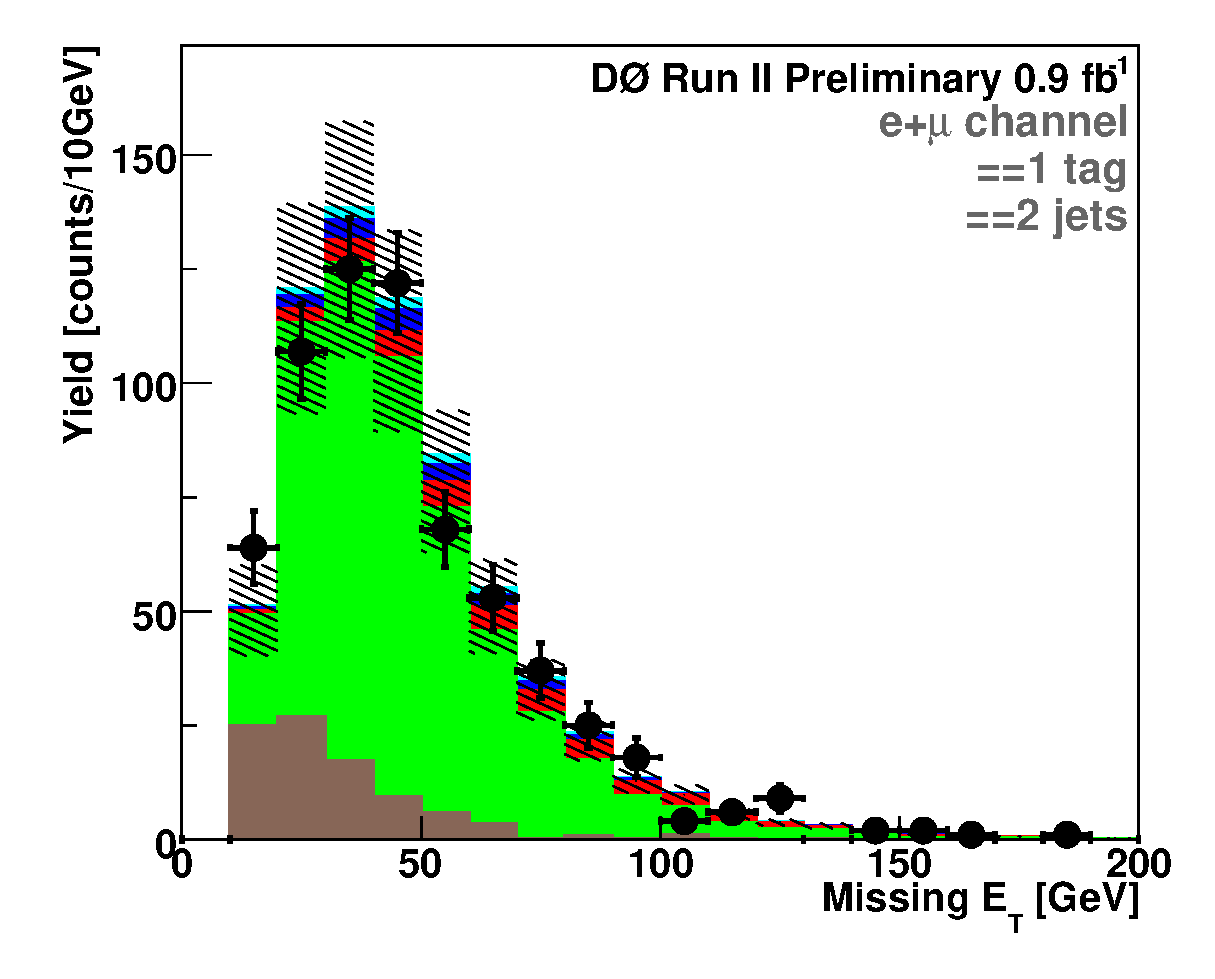
\includegraphics[width=0.32\textwidth]{eps/DataBackground/EMU/emu_EqOneTag_EqTwoJet_MissingEt.eps}
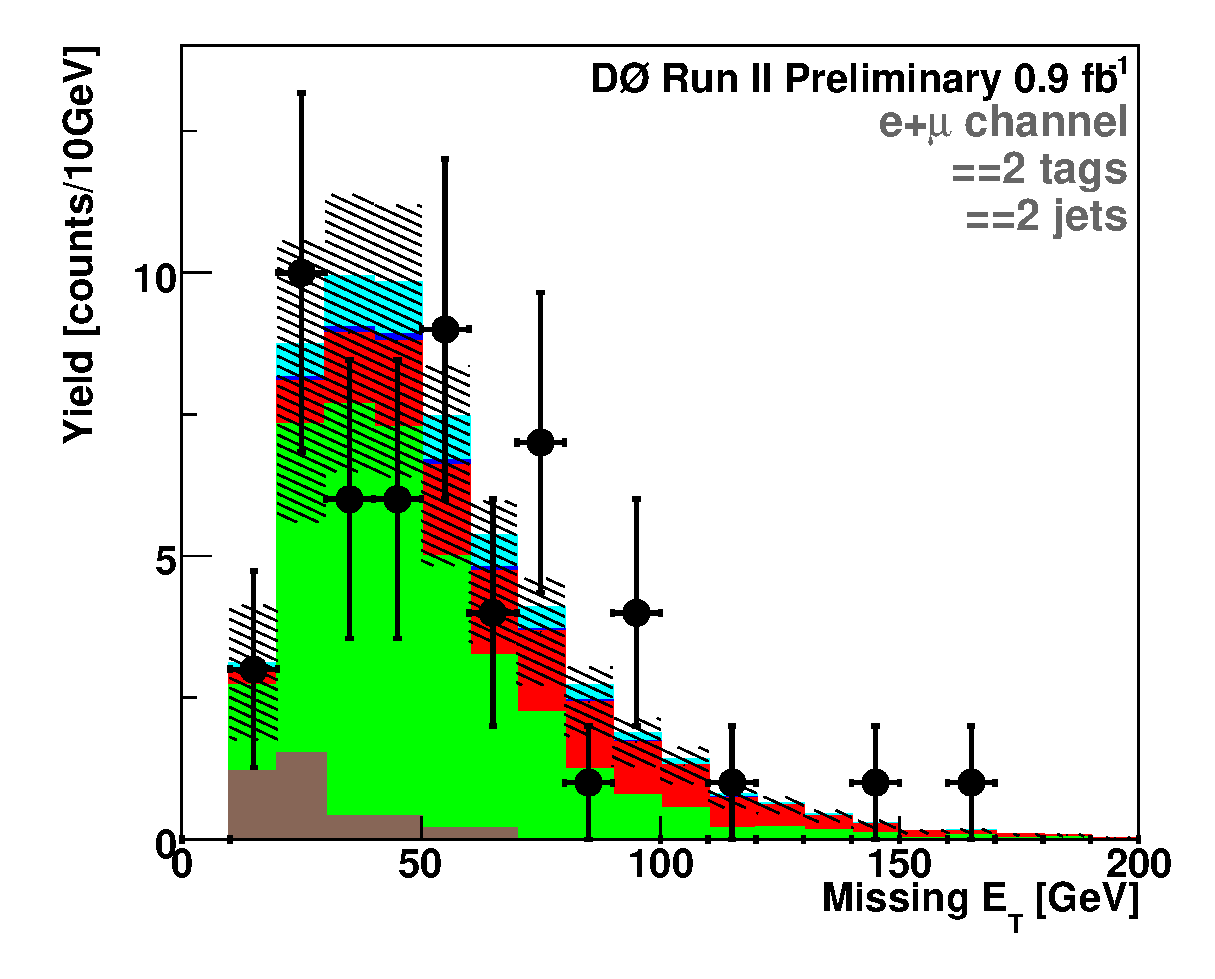
\includegraphics[width=0.32\textwidth]{eps/DataBackground/EMU/emu_EqTwoTag_EqTwoJet_MissingEt.eps}
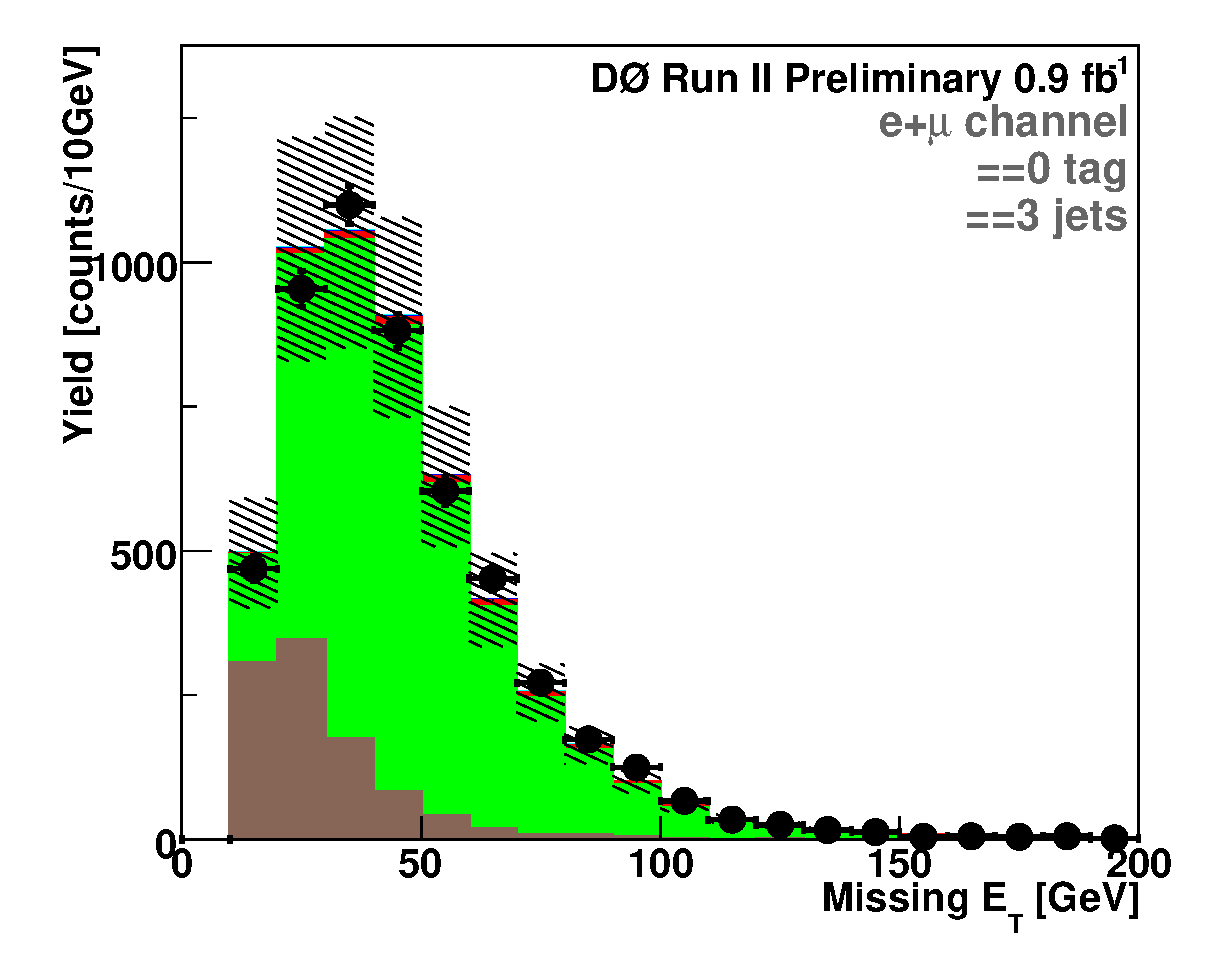
\includegraphics[width=0.32\textwidth]{eps/DataBackground/EMU/emu_EqZeroTag_EqThreeJet_MissingEt.eps}
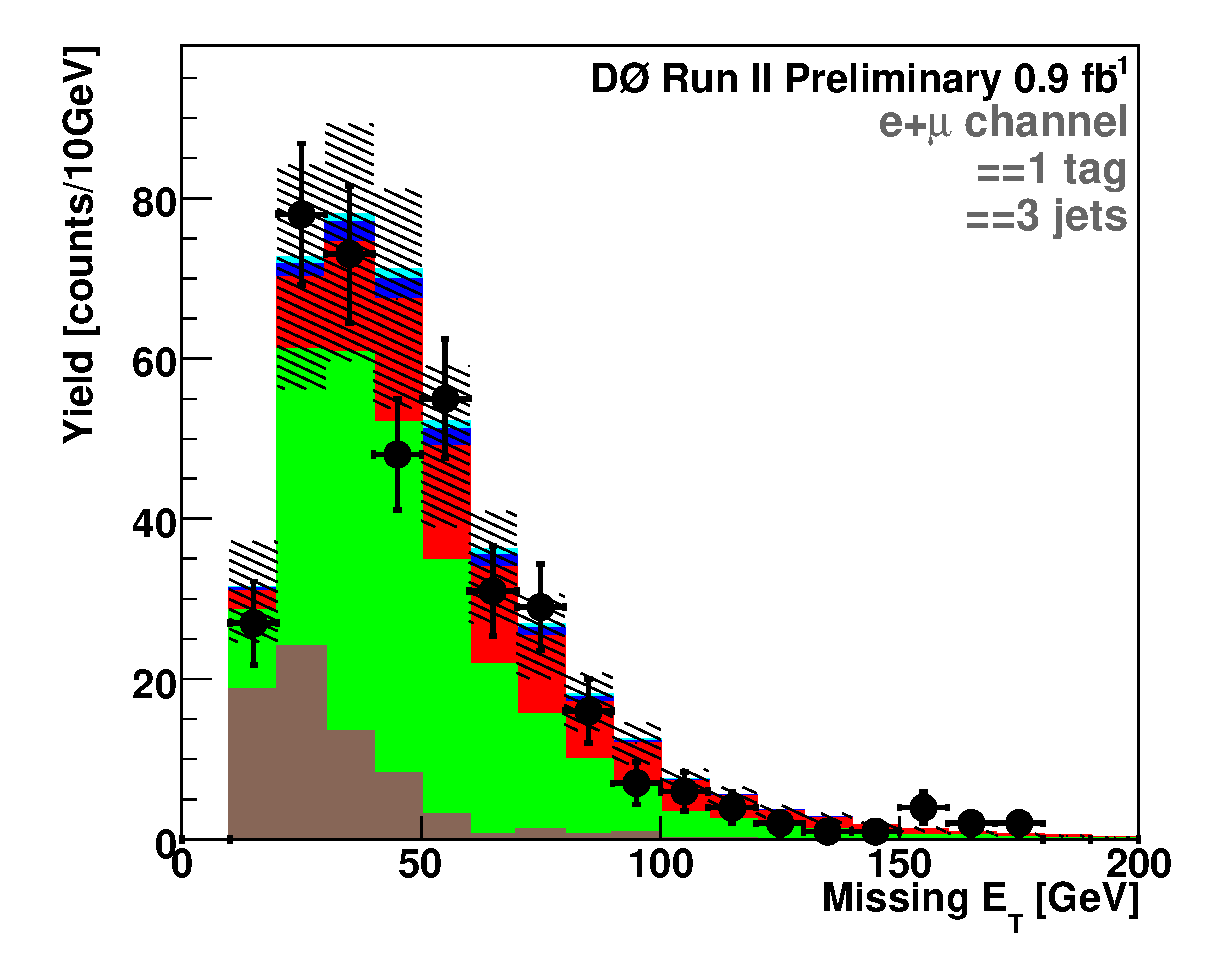
\includegraphics[width=0.32\textwidth]{eps/DataBackground/EMU/emu_EqOneTag_EqThreeJet_MissingEt.eps}
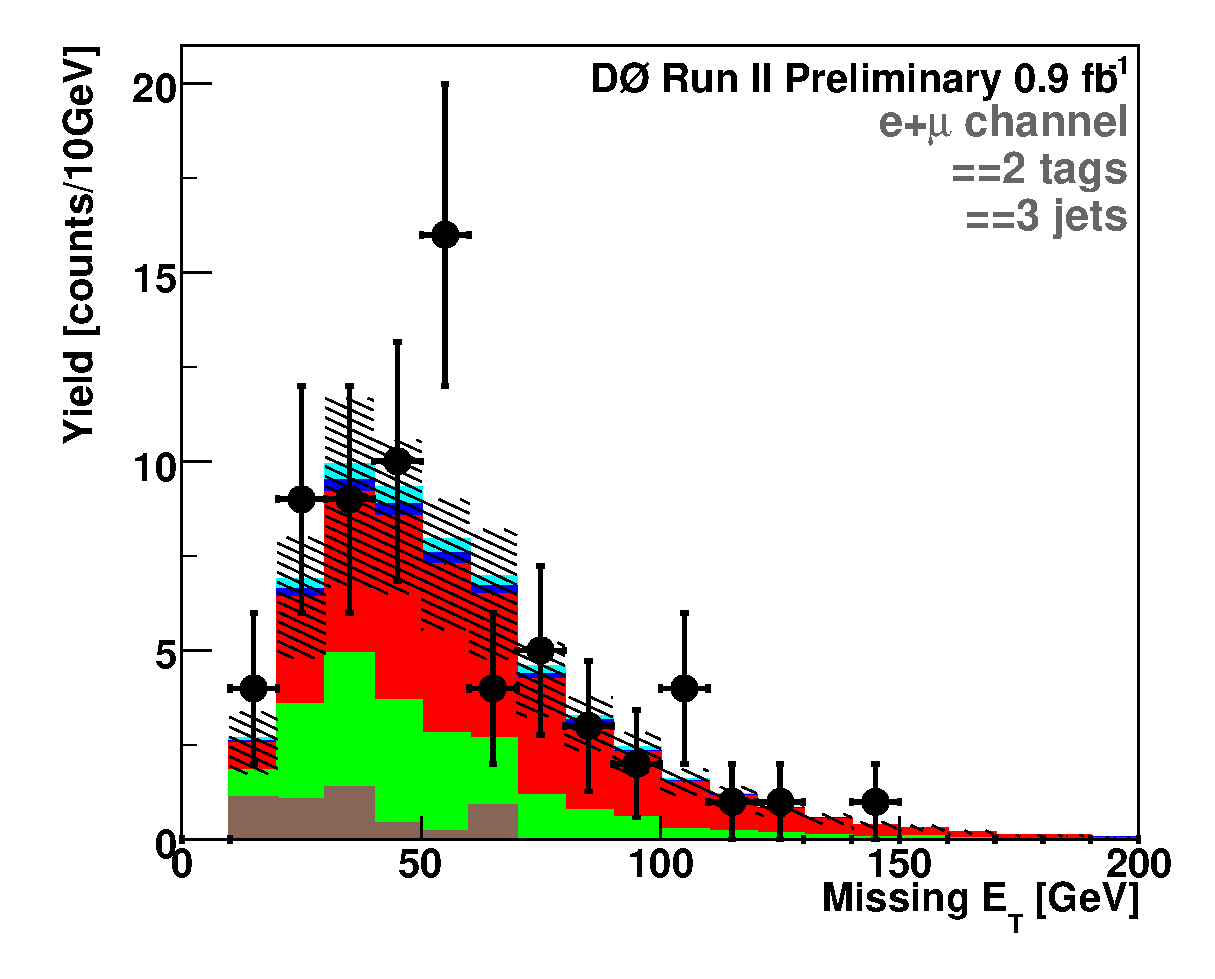
\includegraphics[width=0.32\textwidth]{eps/DataBackground/EMU/emu_EqTwoTag_EqThreeJet_MissingEt.eps}
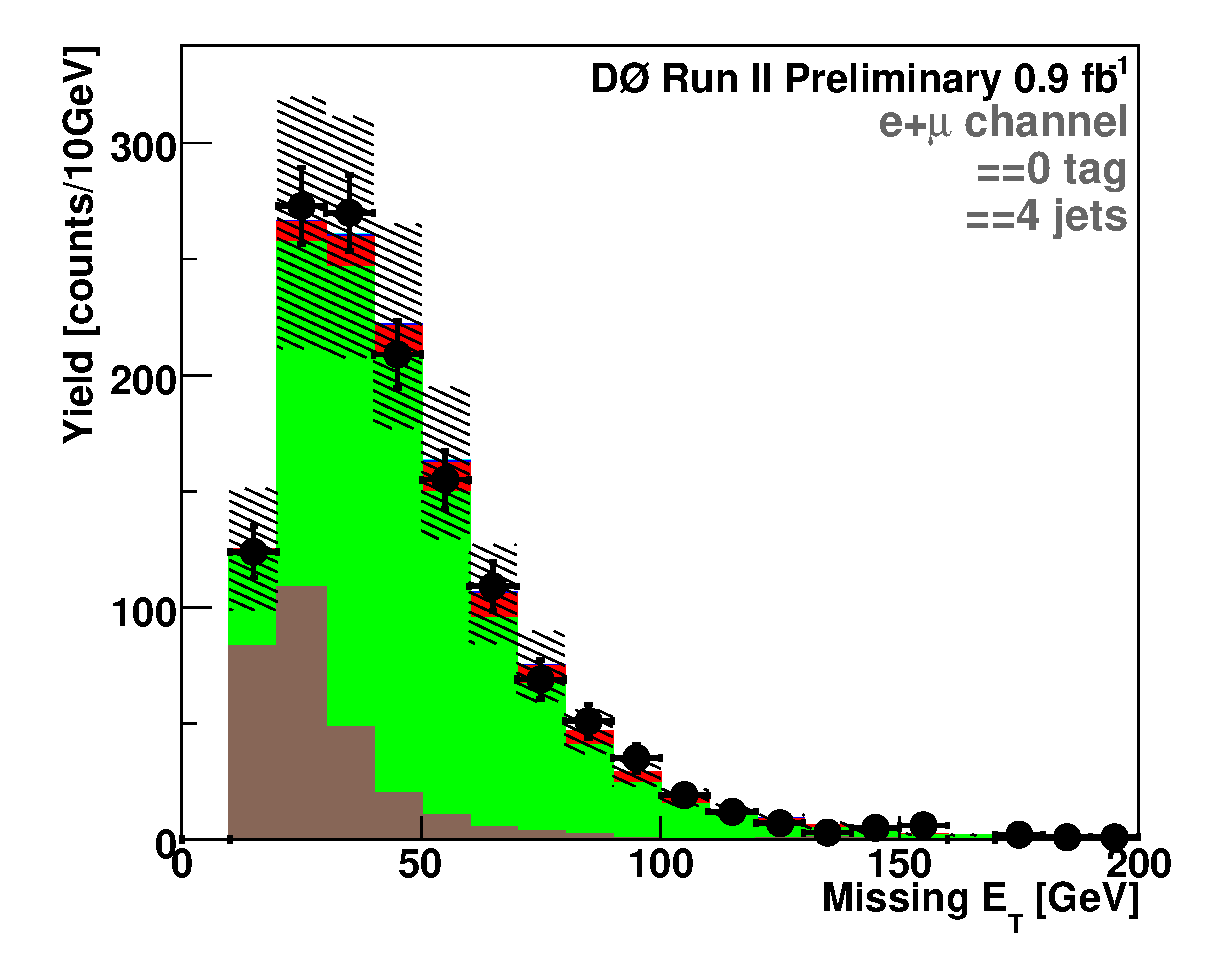
\includegraphics[width=0.32\textwidth]{eps/DataBackground/EMU/emu_EqZeroTag_EqFourJet_MissingEt.eps}
\includegraphics[width=0.32\textwidth]{eps/DataBackground/EMU/emu_EqOneTag_EqFourJet_MissingEt.eps}
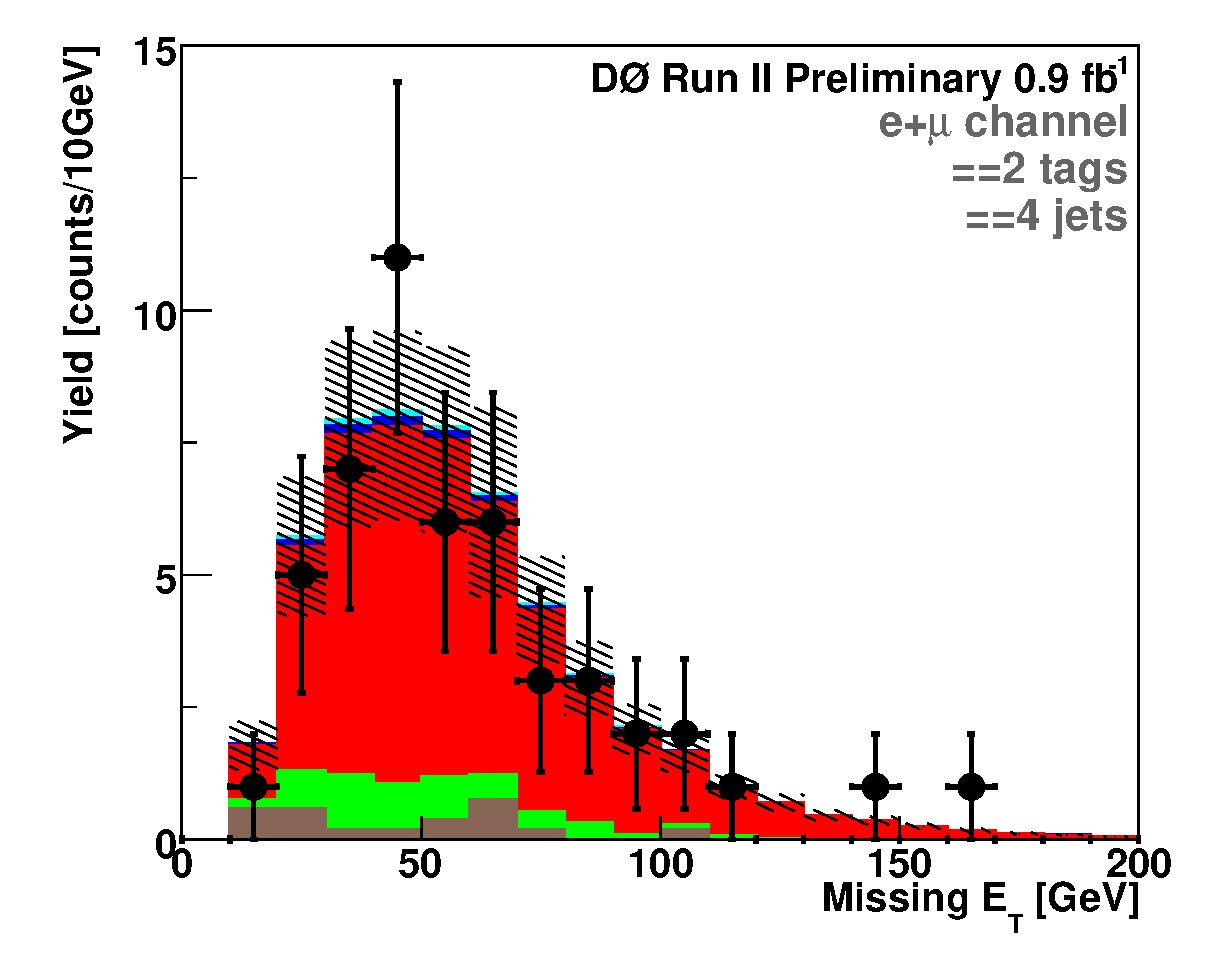
\includegraphics[width=0.32\textwidth]{eps/DataBackground/EMU/emu_EqTwoTag_EqFourJet_MissingEt.eps}
\end{center}
\vspace{-0.1in}
\caption{Missing $E_{T}$ distributions. Upper row: events with 2 jets, Middle row: events with 3 jets, Lower row: events with 4 jets. Left column: events before $B$-tagging, Middle row: events with one selected $B$-jet, Right column: events with two selected $B$-jets~\cite{singletopnote}.}
\label{MissingEt}
\end{figure}






